\chapter{Implementation} \label{ch:implementation}
\markboth{Implementation}{}

\paragraph{}

At the core of this thesis, rests the implementation of the above mentioned architecture. In this Chapter, we are going to introduce the protocols and platforms that were used for the implementation, the scenario of the use-case and finally provide a walkthrough of our approach, noting the architecture modules that were actually implemented.

The proposed architecture of Chapter \ref{ch:system-architecture} was implemented with several assumptions, so as to create a proof of concept for a narrow aspect of the design. Moreover, as presented in Chapter \ref{ch:system-architecture}, the architecture is highly affected by the used technologies (i.e EdgeX, Filecoin, etc)

\section{Scenario}

The scenario that was chosen for the implementation of our reference use-case is fairly simple. We assume an edge device that handles a sensor which is connected through LoRa. This edge device has entered into a service contract with another edge device which also supports the LoRa protocol. In our scenario, EdgeA has a failure and EdgeB detects the failure, activates the contract and kickstarts the services in order to control the sensor.

In the implementation, each Edge consists of a Raspberry Pi 3 and a Lorank8 (Beaglebone Black) that are networked over LAN. Although they are two distinct hardware boards, we model our Edge as the combination of those two. Each Edge device has therefore it’s own LoRa gateway, both in terms of software (i.e packet forwarder) and in terms of hardware.


\subsection{Hardware}

For the Edge device, a combination of two hardware edges was used as neither provided adequate performance for our implementation on its own. We started with a Raspberry Pi 3 which would house the entirety of the application logic, while Lorank8 (Beaglebone Black) would only function as the gateway component. After verifying that Raspberry pi 3 was inadequate for the array of microservices that we would run, we opted for a distributed architecture, simulating the Edge device as the networked combination of these 2 boards.

Figure \ref{fig:dist_arch} illustrates the distribution of services between the devices, where each polygon is a distinct microservice. In BalenaOS the microservices are containerized, meaning that each polygon is in essence a single container, while in Debian Jessie, the services run natively on the OS without any form of isolation (increased efficiency).

\begin{figure}[h]
    \centering
    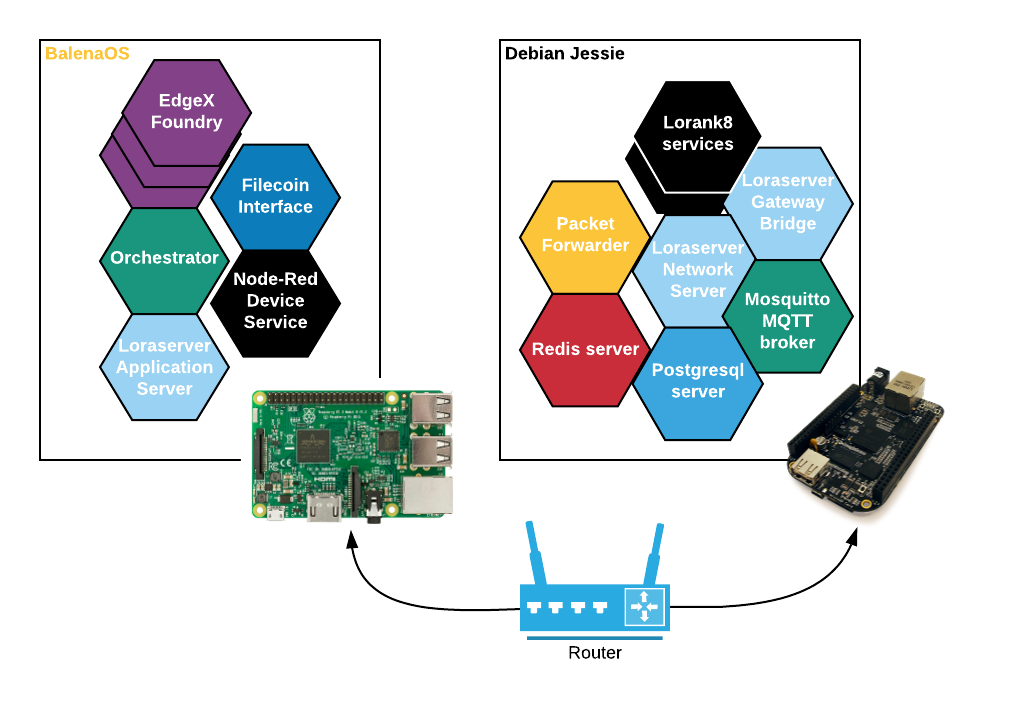
\includegraphics[width=0.9\textwidth]{images/dist_arch_hardware.png}
    \caption{Overview of the distribution of services between the 2 hardware parts of the Edge device}
    \label{fig:dist_arch}
\end{figure}

\subsection{Services}

Moreover, we had to make some assumptions regarding the software and the fault-tolerance mechanism. 

In our scenario it is assumed that the implementation focuses on the handover and not the negotiation process. Thus the marketplace interface, Arbitrator and DMU microservices were removed all-together. Moreover, for matters of efficiency, Filecoin interface and orchestrator were combined in one service, but remain logically decoupled. This means that the two microservices have distinct APIs but are housed in the same program . Finally, the orchestrators of different Edge devices communicate directly, without an Edge2Edge interface intermediary, using HTTP requests and RESTful APIs.

\section{Communication Protocols used in the Implementation}

Before proceeding, we believe it is worth providing an apt description of the communication protocols that are used in the implementation and will be referenced throughout this chapter.

\subsection{MQTT}
\acrfull{mqtt}\cite{mqtt} is one of the most commonly used protocols in the IoT projects and like other internet protocols, it is based on clients and a server. Unlike others, the MQTT makes it easier to implement software and transmit data at a quicker pace, while it also minimizes data packets and consumes less energy. This protocol functions on top of the TCP/IP and it includes a subscriber, a publisher and a broker. The publisher collects the data and sends it to subscribers, using the broker service. It is considerably more power efficient that HTTP.

\subsection{HTTP/REST}
REST, or REpresentational State Transfer, is an architectural style for providing standards between computer systems on the web, making it easier for systems to communicate with each other. REST-compliant systems, often called RESTful systems, are characterized by how they are stateless and separate the concerns of client and server. In the REST architectural style, the implementation of the client and the implementation of the server can be done independently without each knowing about the other (Loosely coupled). Finally, Systems that follow the REST paradigm are stateless, meaning that the server does not need to know anything about what state the client is in and vice versa. When HTTP is used, as is most common, the operations (HTTP methods) available are GET, HEAD, POST, PUT, PATCH, DELETE, CONNECT, OPTIONS and TRACE.

\subsection{gRPC}
gRPC\cite{grpc} is a modern, open source \acrfull{rpc} framework that can run on most computing systems and has clients for most programming languages. It enables client and server applications to communicate transparently, and makes it easier to build connected systems.

Finally, gRPC was firstly developed by Google, uses HTTP/2 as it’s transport-layer protocol and protocol buffers for it’s interface description language. It is also a Cloud Native Computing Foundation (CNCF) project.

\subsection{LoRa}
LoRa (Long Range)\cite{LoRa} is a patented digital wireless data communication IoT technology developed by Cycleo of Grenoble, France. It was acquired by Semtech in 2012, which holds the IP for LoRa transmission methodology. LoRa transmits over license-free sub-gigahertz radio frequency bands like 169 MHz, 433 MHz, 868 MHz (Europe) and 915 MHz (North America). LoRa enables very-long-range transmissions (more than 10 km in rural areas) with low power consumption and low data throughput.
The technology is presented in two parts — LoRa, the physical layer, and; the communication protocol built upon the underlying LoRa physical layer. The communication layer is usually LoRaWAN (Long Range Wide Area Network), an open source communication protocol defined by the LoRa Alliance consortium; Thus, LoRaWAN™ defines the communication protocol and system architecture for the network, while the LoRa® physical layer enables the long-range communication link. LoRa WAN communication protocol ensures reliable communication, secure communication and adds additional headers to the data packets. LoLoRaWAN network architecture is deployed in a star-of-stars topology (vs. mesh topology eg. Zibgee).

The LoRaWAN networks laid out in a star-of-stars topology have base stations relaying the data between the sensor nodes and the network server.
Communication between the sensor nodes and the base stations goes over the wireless channel utilizing the LoRa physical layer, whilst the connection between the gateways and the central server (LoraWAN cloud - network server) is handled over a backbone IP-based network. 

\begin{itemize}
    \item \textbf{Gateways:} At the core of each gateway, runs a packet forwarder\cite{packetfor}. A program that forwards RF packets received by the concentrator to a server (network server) through an IP/UDP link. It also emits RF packets that are sent by the server.
    \item \textbf{Network servers:} They connect to the gateways, de-duplicate data packets (as a packet sent from a sensor might have been picked up by multiple gateways), and then routes them to the relevant application.They can be used for both uplink (i.e. sensor to application) or downlink (i.e. application to sensor) communication. 

\end{itemize}

A reference diagram of a typical LoRaWAN network is shown in figure \ref{fig:LoRa}. In our implementation, we use an open source LoRaWAN project, called loraserver.io.
\clearpage

\begin{figure}[H]
    \centering
    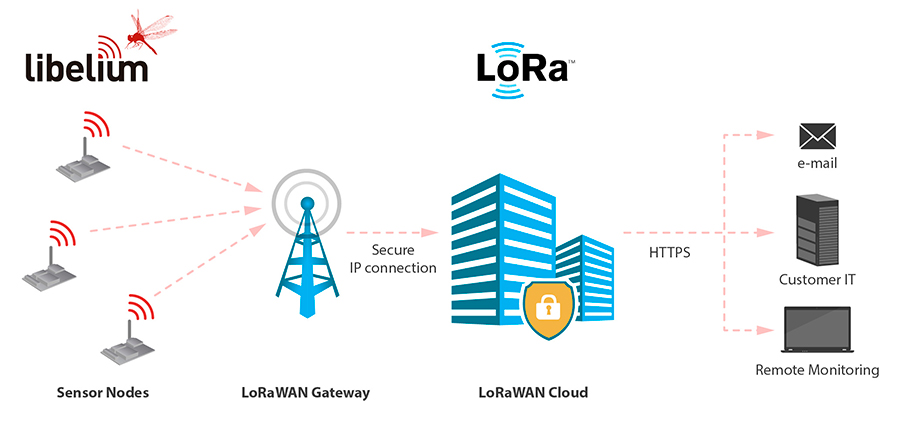
\includegraphics[width=0.9\textwidth]{images/lora_arch.jpg}
    \caption{A LoRa reference architecture, courtesy of Libelium\cite{libelium}}
    \label{fig:LoRa}
\end{figure}

\section{Platforms used in the Implementation}
Having established the communication protocols that are used in the implementation, we now turn our focus on the platforms that were used to develop the implementation. These platforms were not mentioned in the architecture Chapter as they do not consist building blocks of the architecture, but rather choices for our proof of concept. The description of platforms that were presented in Architecture Chapter \ref{ch:system-architecture} will be omitted. Firtly, we believe it’s important to underline the selection criteria for our implementation choices in order to help the reader make informed decisions in case he wants to replicate our implementation.

Criteria, in order of importance:
\begin{enumerate}
    \item Speed of development:  Since we only wish to create a proof of concept for a narrowly defined part of the architecture, the speed of development is our primary drive.
    \item Complexity: Software engineering and robustness of the solutions are out of scope, we used solutions and programming languages that offer the minimum complexity.
\item Performance: We strive to optimise the performance of the chosen solutions due to the restricted nature of the chosen Edge hardware platform.

\end{enumerate}
\noindent
Taking into account the above mentioned criteria, we chose these solutions for our implementation:

\bigskip
\noindent
\textbf{Edge Hardware:} Raspberry pi 3 B+
\newline
\textbf{Edge platform:} Balena
\newline
\textbf{Edge core:} EdgeX Foundry
\newline
\textbf{LoRa Gateway:} Lorank8
\newline
\textbf{LoRa Sensor:} Arduino with Lora/GPS shield
\newline
\textbf{LoRaWAN suite (Gateway, Network-Server, Application Server):} loraserver.io
\newline
\textbf{Software Development:} NodeRed, Python Flask
\newline
\textbf{Development Tools:} Visual Studio Code, Postman, Terminal

\subsection{Raspberry pi 3 B+}

Raspberry pi 3 B+ \cite{rpi3} uses the Broadcom BCM2837B0 system-on-chip (SoC) which includes four high-performance Cortex-A53 (ARMv8) 64-bit processing cores running at 1.4 GHz with 32kB Level 1 and 512kB Level 2 cache memory, a VideoCore IV graphics processor, and is linked to a 1GB LPDDR2 (900 MHz) memory module on the rear of the board. Raspberry pi is in essence a small linux computer and was chosen for the wealth of available software and it’s enormous community, it is considered as the de-facto development \& educational board for IoT Edge linux computers. The board along with it's main components is shown in Figure \ref{fig:Raspberrypi3}.

\begin{figure}[h]
    \centering
    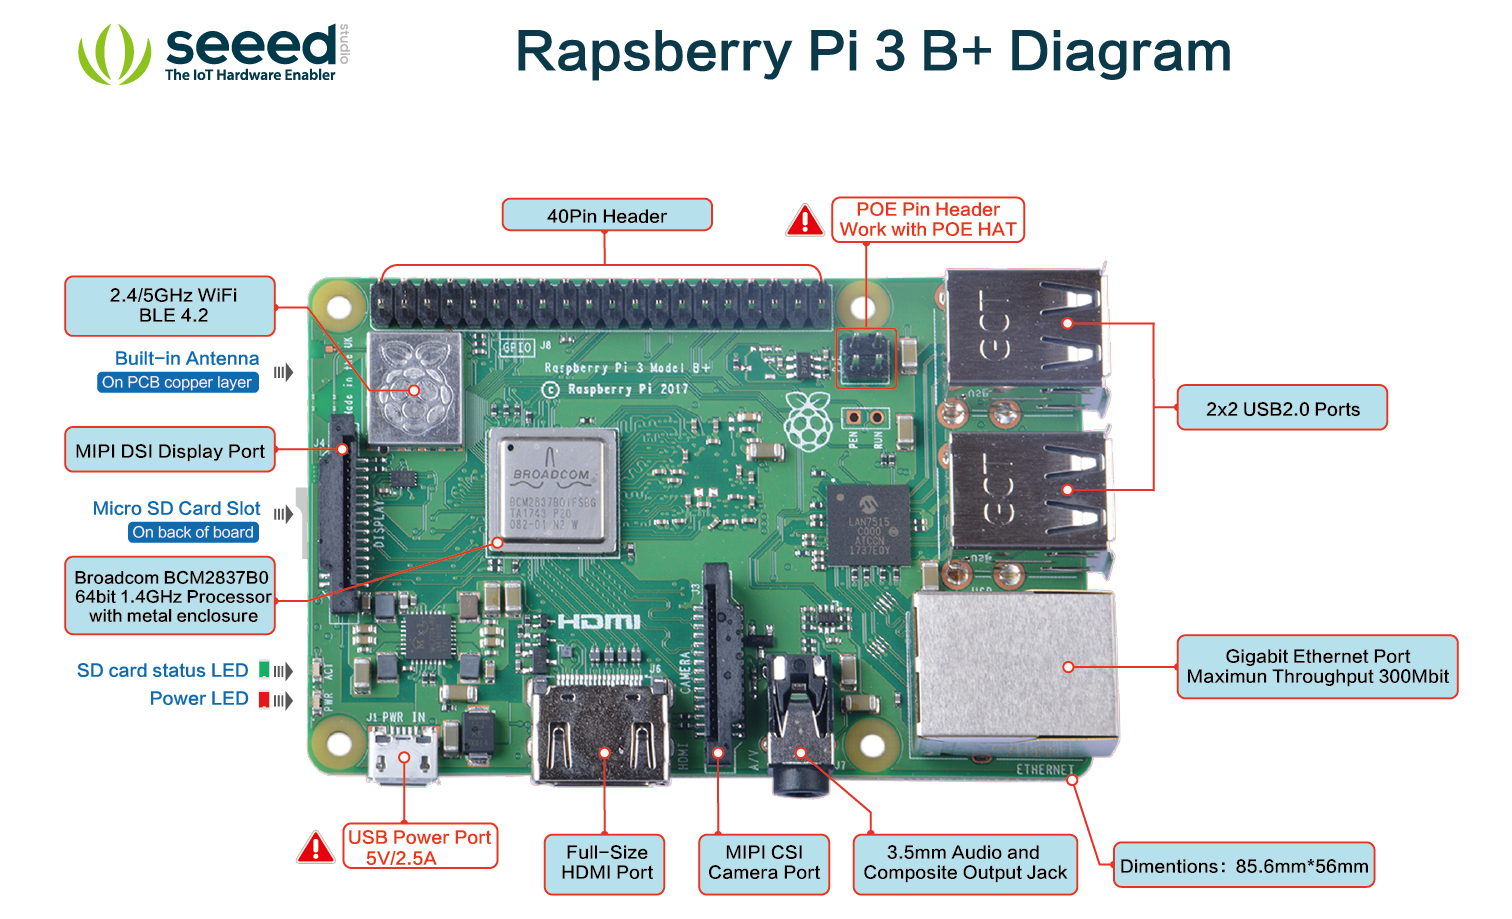
\includegraphics[width=1\textwidth]{images/raspberrypi3.jpg}
    \caption{Raspberry pi 3 B+ and it's components, courtesy of Seeed studio \cite{rpiseeed}}
    \label{fig:Raspberrypi3}
\end{figure}

\subsection{Lorank8}
The Lorank8\cite{lorank8} is a LoRa Gateway with professional specifications. With almost 50 DSP pipes on board it processes 8 LoRa transmissions simultaneously. This enables the connection with several tens of thousands end nodes around the gateway. Moreover, with a sensitivity of -138 dBm and a maximum power of 500 mW it can easily reach the most distant nodes. The hardware is based on the high quality radio board of IMST and the open source Beagle Board\cite{beaglebone}.  The software is open sourced and it works out-of-the-box, enabling us to setup the gateway to our specifications in a short period of time. We opted to enclose Lorank8 in an weather resistant IP67 enclosure, as shown in Figure \ref{fig:Lorank8}.

\begin{figure}[h]
    \centering
    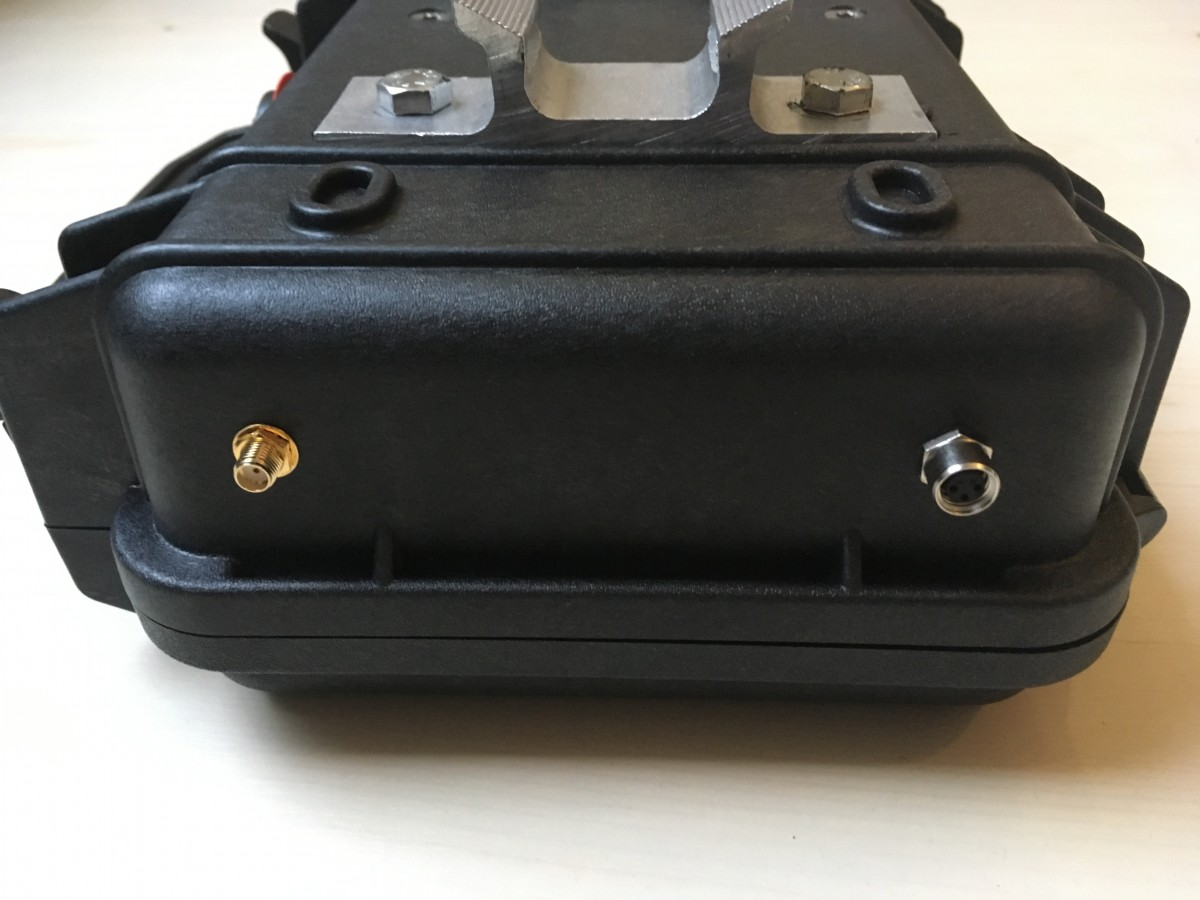
\includegraphics[width=0.5\textwidth]{images/lorank8.jpg}
    \caption{The Lorank8 encased in a weather resistant enclosure \cite{lorank8}}
    \label{fig:Lorank8}
\end{figure}


\subsection{Arduino with LoRa/GPS shield}

Arduino\cite{arduino} is an open source platform that can be used to design various electronic projects. It’s flagship product, Arduino UNO, is based on microcontroller ATmega 328P. It has 14 digital input/output pins (of which 6 can be used as PWM outputs), 6 analog inputs, a 16 MHz quartz crystal, a USB connection, a power jack, an ICSP header and a reset button. It is shown in Figure \ref{fig:Arduino}. Arduino uses its own IDE(Integrated Development Environment),shown in Figure \ref{fig:Arduino_ide}, and is programmed in a simplified version of C++.

The Dragino LoRa/GPS Shield \cite{dragino} is an expansion board for LoRa/GPS for using with the Arduino. It is composed of a LoRa/GPS Shield motherboard and Lora BEE. In the LoRa part, the LoRa/GPS Shield is based on the SX1276/SX1278 transceiver.The transceivers of the LoRa/GPS Shield incorporate the LoRa long range modem that provides ultra-long range spread spectrum communication and high interference immunity whilst minimising current consumption. LoRa also provides significant advantages in both blocking and selectivity over conventional modulation techniques, solving the traditional design compromise between range,interference immunity and energy consumption.

\begin{figure}[H]
    \centering
    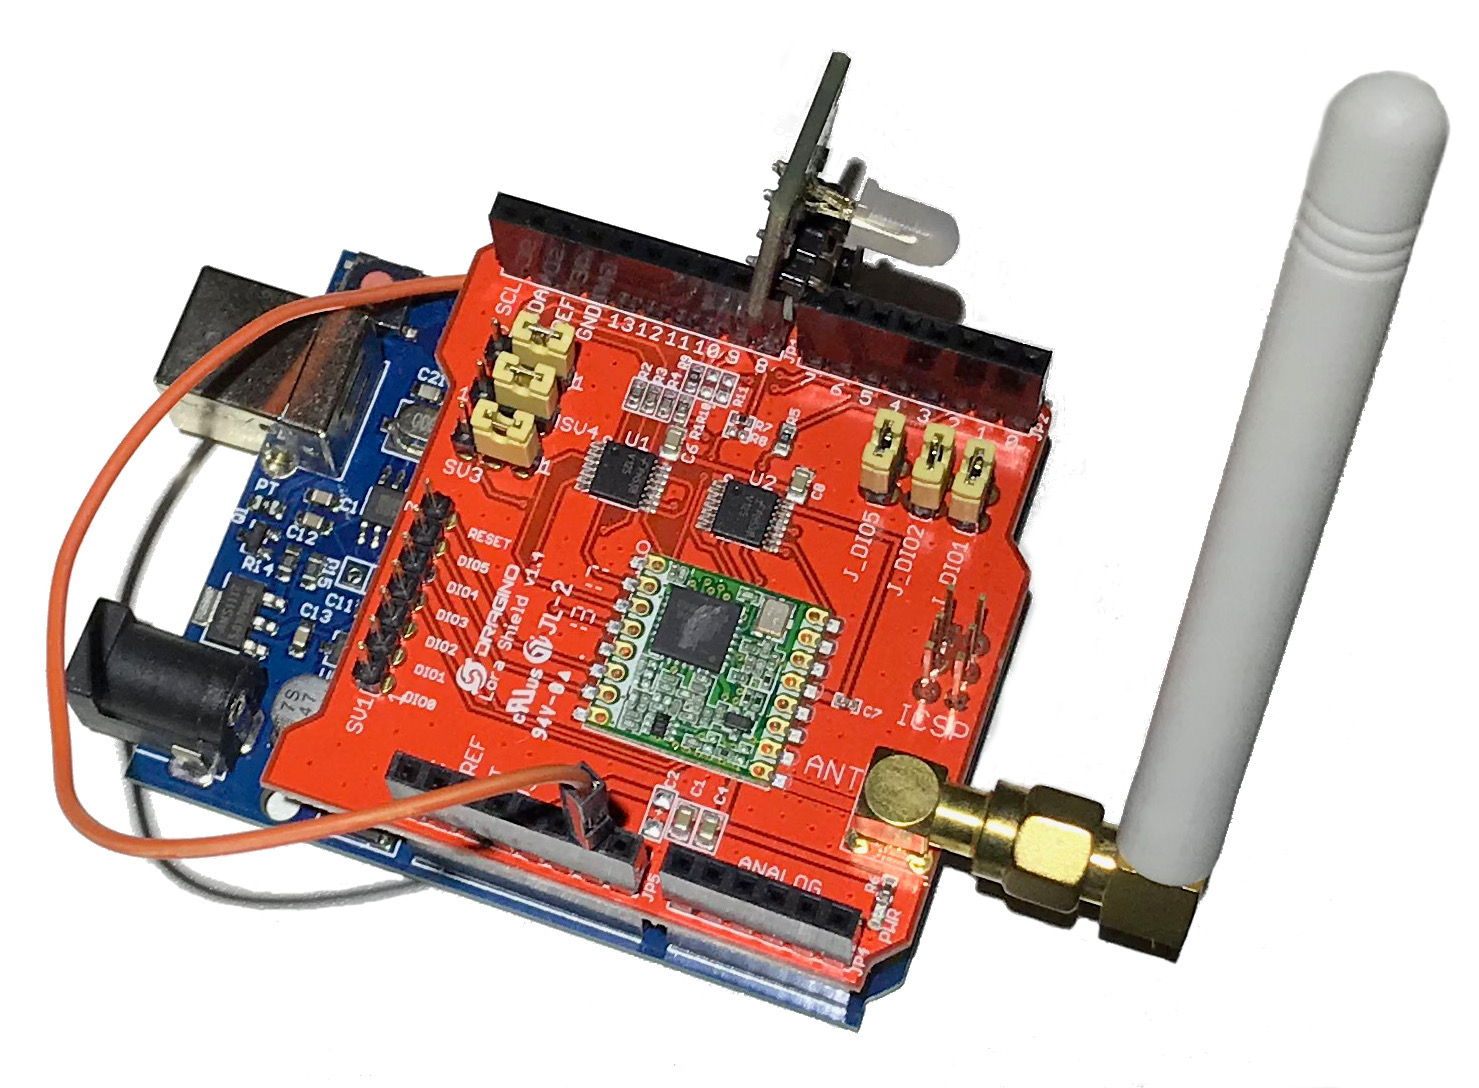
\includegraphics[width=0.4\textwidth]{images/arduino.jpg}
    \caption{an Arduino UNO with the Draggino LoRa/GPS shield \cite{dragino}}
    \label{fig:Arduino}
\end{figure}

\begin{figure}[H]
    \centering
    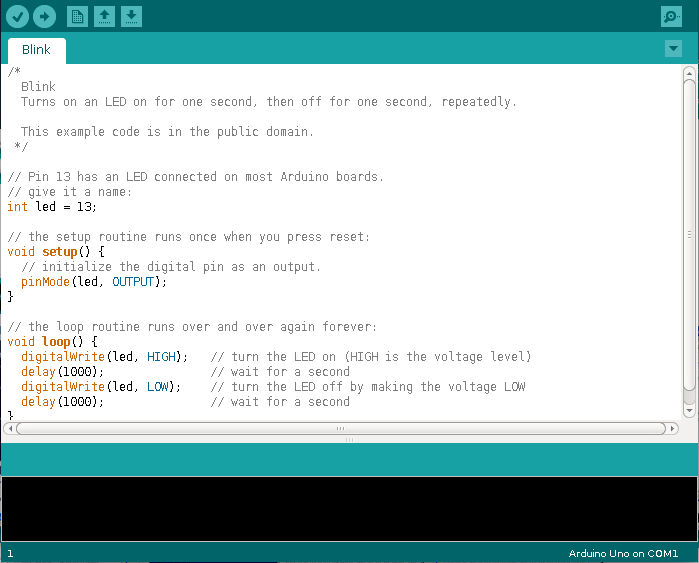
\includegraphics[width=0.5\textwidth]{images/arduino_ide.png}
    \caption{Arduino are easily programmed using the Arduino IDE \cite{arduino}}
    \label{fig:Arduino_ide}
\end{figure}

\subsection{loraserver.io}

The LoRa Server project\cite{loraserver} is an open-source set of applications which is placed between the gateways which receive messages from the nodes to just before the applications receiving the data. It provides mechanisms for managing the gateways on the LoRa network, the applications supported, and the devices associated with the applications.
The project is designed to be used in a very flexible manner and consists of 3 main components:

\begin{itemize}
    \item Gateway Bridge: LoRa Gateway Bridge is a platform which converts the packets outputed by the LoRa packet-forwarder into loraserver.io compatible format (JSON, Protobuf). It receives the UDP packets from the forwarder and outputs an MQTT stream at a connected MQTT broker.
    \item Network server: The network server is responsible for the functionality needed by a network-server (i.e de-duplication of packets, management of the LoRaWAN mac-layer and the handling of uplink/downlink data transmissions).
    \item Application Server: It is responsible for the device inventory, handling join requests and the encryption of application payloads. It offers a web interface and a RESTful and gRPC API.

\end{itemize}
Figure \ref{fig:LoRaserver} illustrates the aforementioned architecture of the LoRaserver project.

\begin{figure}[h]
    \centering
    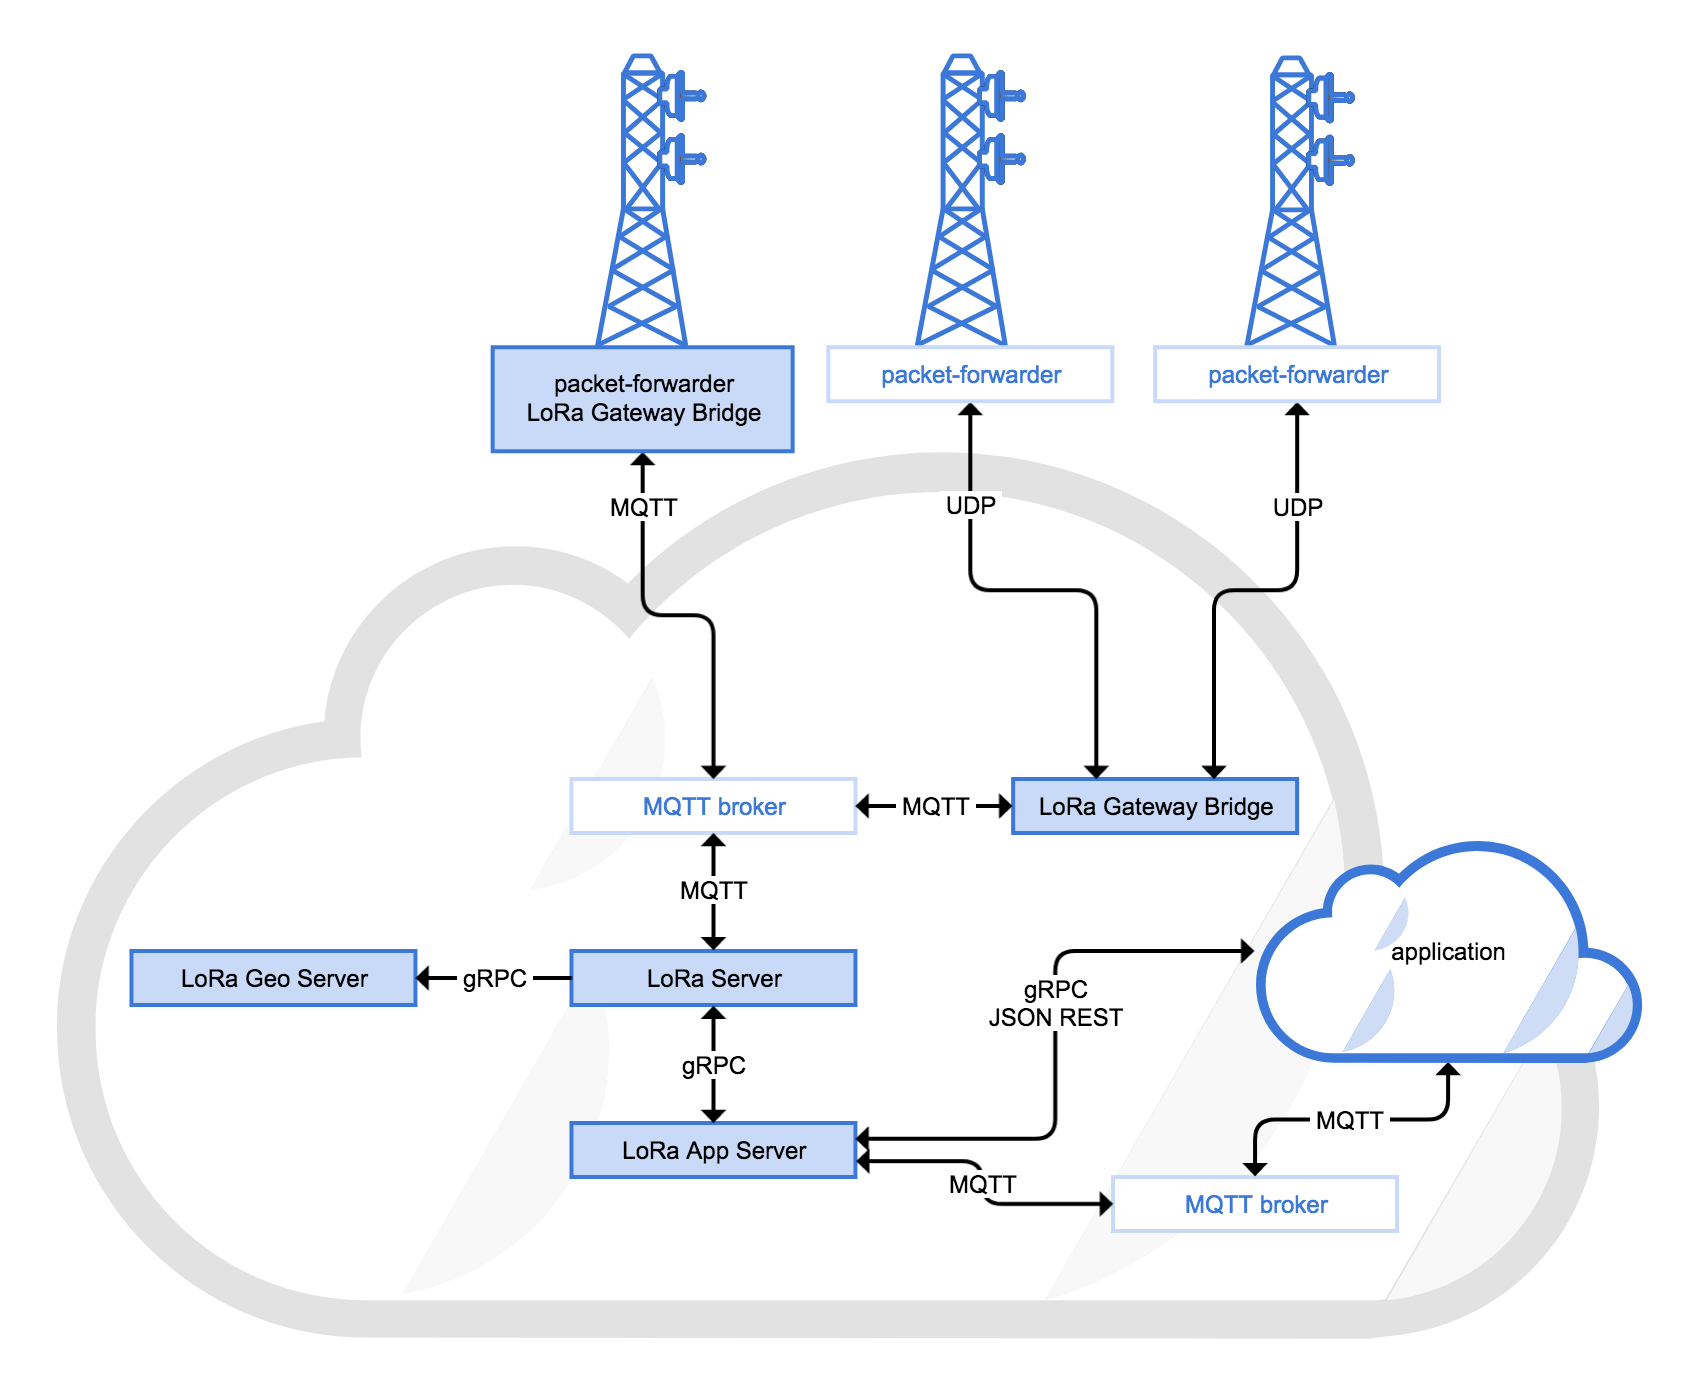
\includegraphics[width=0.8\textwidth]{images/loraserver-arch.png}
    \caption{Overview of the loraserver.io project architecture \cite{loraserver}}
    \label{fig:LoRaserver}
\end{figure}

\subsection{Node-RED}
Node-RED\cite{nodered} is a flow-based programming tool originally developed by IBM’s Emerging Technology Services and is now part of the JS Foundation. Flow-based programming was invented by J. Paul Morrison in the 1970s and is a way of describing an application’s behavior as a network of black-boxes. Each black box has a number of inputs and a number of outputs. It takes the data, performs some abstract computation and then passes the data to the next box.

Node-Red makes programming more accessible to users since it offers the flexibility to create applications, mainly around the IoT domain, without having to worry about a number of common programming hurdles, such as concurrency, execution, etc.  

We used Node-Red to develop various components that could be easily modeled as flows (e.g API resources). Moreover, Node-Red allowed us to focus exclusively on the functionality of the service that was developed. When developing in Node-Red, the developer uses the web GUI to create flows and connect the various nodes. Moreover, it offers customizability by enabling the user to create arbitrary nodes using Javascript. The default data structure that is passed from each node to the next one is named “\textit{msg}” while usually the main input and output component is the attribute “\textit{msg.payload}”. The flows are saved in a json file. An example of a flow is seen in the web GUI  in Figure \ref{fig:nodered}.

On the downside, it’s performance was not adequate for our Edge requirements, since, as of version 0.2.0, it consumes considerable Memory, even for the lightest of functionality. This renders it less favorable versus a python flask script, that has relatively the same learning curve but is considerable more efficient for small scale deployment.

Nevertheless, it’s an ideal tool for proof-of-concepts, due to ease of development, small learning curve and it's immense scalability since it is build on top of a Node.js core.

\begin{figure}[H]
    \centering
    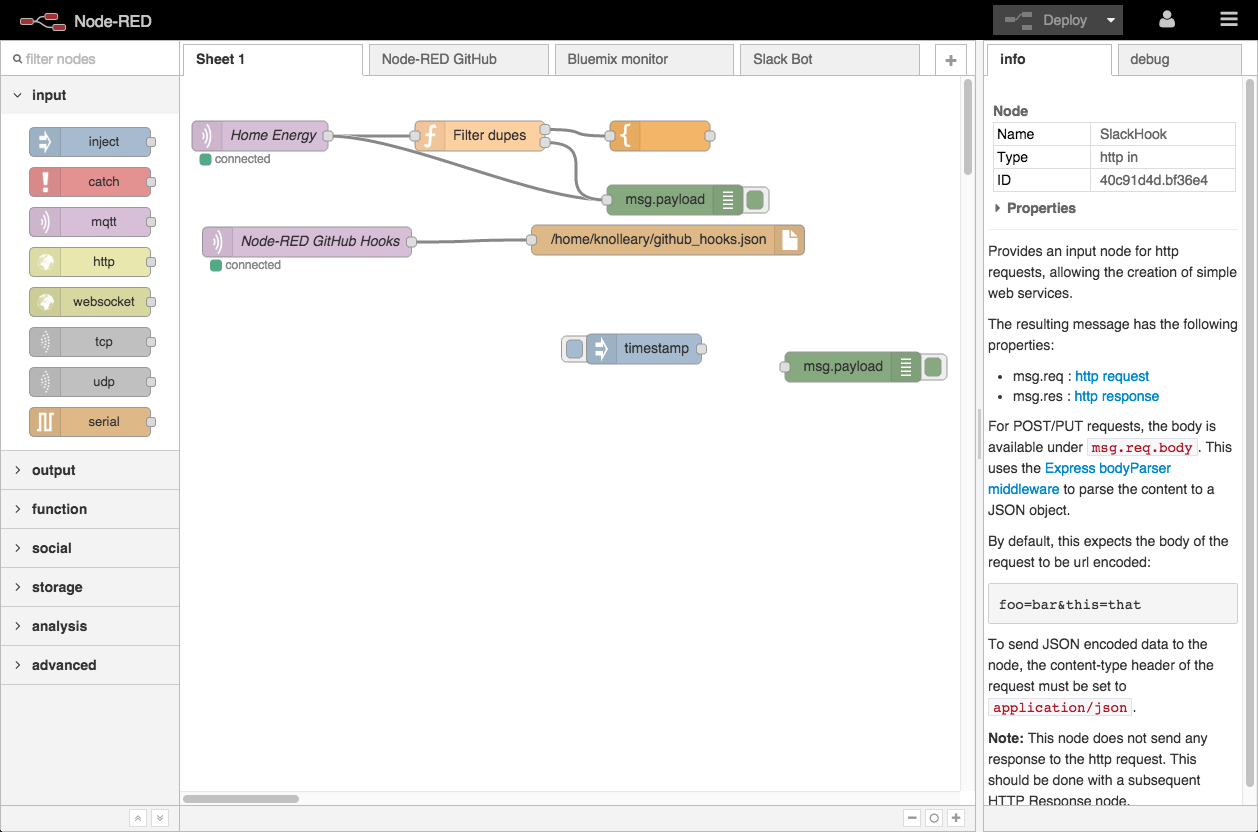
\includegraphics[width=0.8\textwidth]{images/nodered_gui.png}
    \caption{The node-RED web editor GUI \cite{nodered}}
    \label{fig:nodered}
\end{figure}
\newpage

\subsection{Python-Flask framework}

\subsubsection{Python}
Python\cite{python} is a general-purpose programming language that can be used on any modern computer operating system. It can be used for processing text, numbers, images, scientific data and just about anything else you might save on a computer. It is used daily in the operations of the Google search engine, the video-sharing website YouTube, NASA and the New York Stock Exchange.

Python is considered one of the easiest languages to master and understand and is built with ease of use at mind. For that reason, it is mainly used for the speed of development it offers and the small learning curve, while also boasting a huge ecosystem with a wealth of available libraries and frameworks. It is one of the most famous languages to develop the first versions of a product as it is easy to update and change various parts, before converting the stack to a more stable and strictly formatted enterprise solution, such as Java. Python is also the de-facto language used in prototyping and DIY projects, as also for most projects on Raspberry Pi, while it is worth mentioning that lately Node.js and Golang are quickly rising as languages that offer ease of development, namely for web applications (NodeJS) and more generic applications (Golang).

For these reasons, we opted to develop on python a part of the implementation. Since the microservices that we would develop are API based, a web framework was chosen to facilitate us even more. 

\subsubsection{Flask}
Flask\cite{flask} is a lightweight WSGI web application framework. It is designed to make getting started quick and easy, with the ability to scale up to complex applications. It began as a simple wrapper around Werkzeug and Jinja and has become one of the most popular Python web application frameworks. It’s main attribute, is the ease of use, as shown by the “\textit{hello world}” application in Figure \ref{fig:python}. This application shows "Hello, World!" on localhost port 5000 in a web browser when run with the following simple command: \texttt{python app.py}. 

\begin{figure}[H]
    \centering
    \begin{minted}[%
 breaklines,
 mathescape,
 linenos,
 numbersep=5pt,
 frame=single,
 numbersep=5pt,
 xleftmargin=0pt
 ]
{python}
from flask import Flask
app = Flask(__name__)

@app.route('/')
def hello_world():
    return 'Hello, World!'

if __name__ == '__main__':
    app.run()

\end{minted}
    \caption{A flask "hello world" program}
    \label{fig:python}
\end{figure}

\section{Development Tools}
\begin{enumerate}
    \item \textbf{Visual Studio Code:} It is an open-source text-editor\cite{visual} that is easy to use and offers extensive modularity with a wealth of add-ons. It also supports minor IDE-like functionalities, such as debugging, linting, source control, etc. It was used as the main medium to develop the implementation, mainly the python script.
    \item \textbf{Postman:} It is a powerful HTTP client for testing web services\cite{postman}. Postman makes it easy to test, develop and document APIs by allowing users to quickly put together both simple and complex HTTP requests. We used Postman to test EdgeX foundry API as also to test the APIs of the solutions we developed.
\end{enumerate}

\section{Setting up the implementation platforms}
Having established the protocols, platforms and tools that were used to develop this implementation, it is now pertinent to setup the development environment and present a walkthrough on the setup of all the platforms and systems. Afterwards, we will describe the implementation in regards to the architecture, the simplifications that we have made and finally we will talk about the implemented Edge Modules.

The platform was developed on macOS, a unix based system that is akin to Linux and is developed by Apple Inc. The computer is connected to the same LAN as the hardware that was used in the implementation in order to facilitate debugging and deployment. Bash was used as the terminal application of choice and the source code mentioned throughout the implementation is available on github\cite{github-sources}. 
The rest of the implementation walkthrough assume that the implementation replication will be conducted on either a Linux or macOS computer and thus only relevant commands and  software are used. Although Windows replication will not be challenging, the reader will have to research the appropriate tools, software platforms and methods.

\subsection{Balena Setup}

The setup of the balena platform is really simple, as the documents are very explicit\cite{balenaintro}.  Note that when choosing the platform, the user needs to select “Raspberry pi 3 (64 bit OS)”. The Raspberry pi 3 will be featured with the aarch64 version of Balena, still in Beta, as it is needed for the EdgeX to function properly. Aarch64 is the 64bit version of the OS while armv7 (which is default for Raspberry platforms) is 32bit. Thankfully, Raspberry pi 3 supports both OS architecture (but earlier Raspberry pi versions don’t).

The Raspberry should now appear in the application page, shown in Figure \ref{fig:balena_app}. If the user clicks on the device, it will be brought to the dashboard, where the user can overview the services running on the device, the logs the device outputs and also connect to a shell, either to the hostOS, the supervisor container or any user-defined containers. The device view is shown in Figure \ref{fig:balena_device}. We invite the users to playtest balena in order to get comfortable with the platform before proceeding to the rest of the walkthrough. Please note that the “git” related commands shown in the official balena documents, while still functional, are being slowly replaced by balena CLI\cite{balenacli} which is available for both Windows, macOS and Linux.
\newpage
\begin{figure}[H]
    \centering
    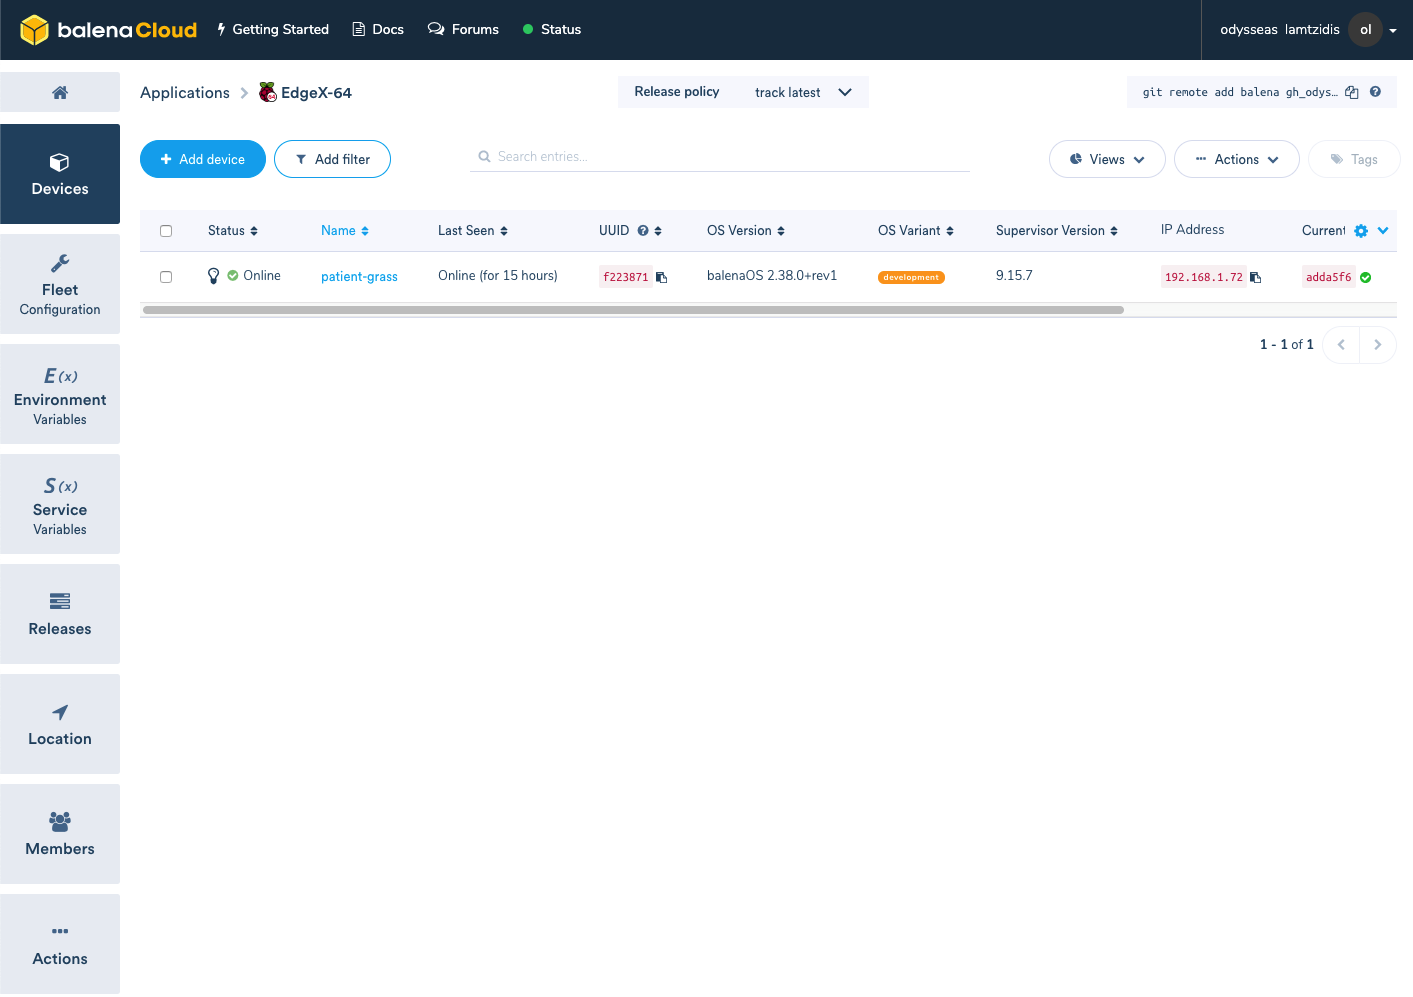
\includegraphics[width=0.9\textwidth]{images/balena_apps.png}
    \caption{Balena Dashboard: The application view where all the devices that belong to the application are shown}
    \label{fig:balena_app}
\end{figure}\begin{figure}[H]
    \centering
    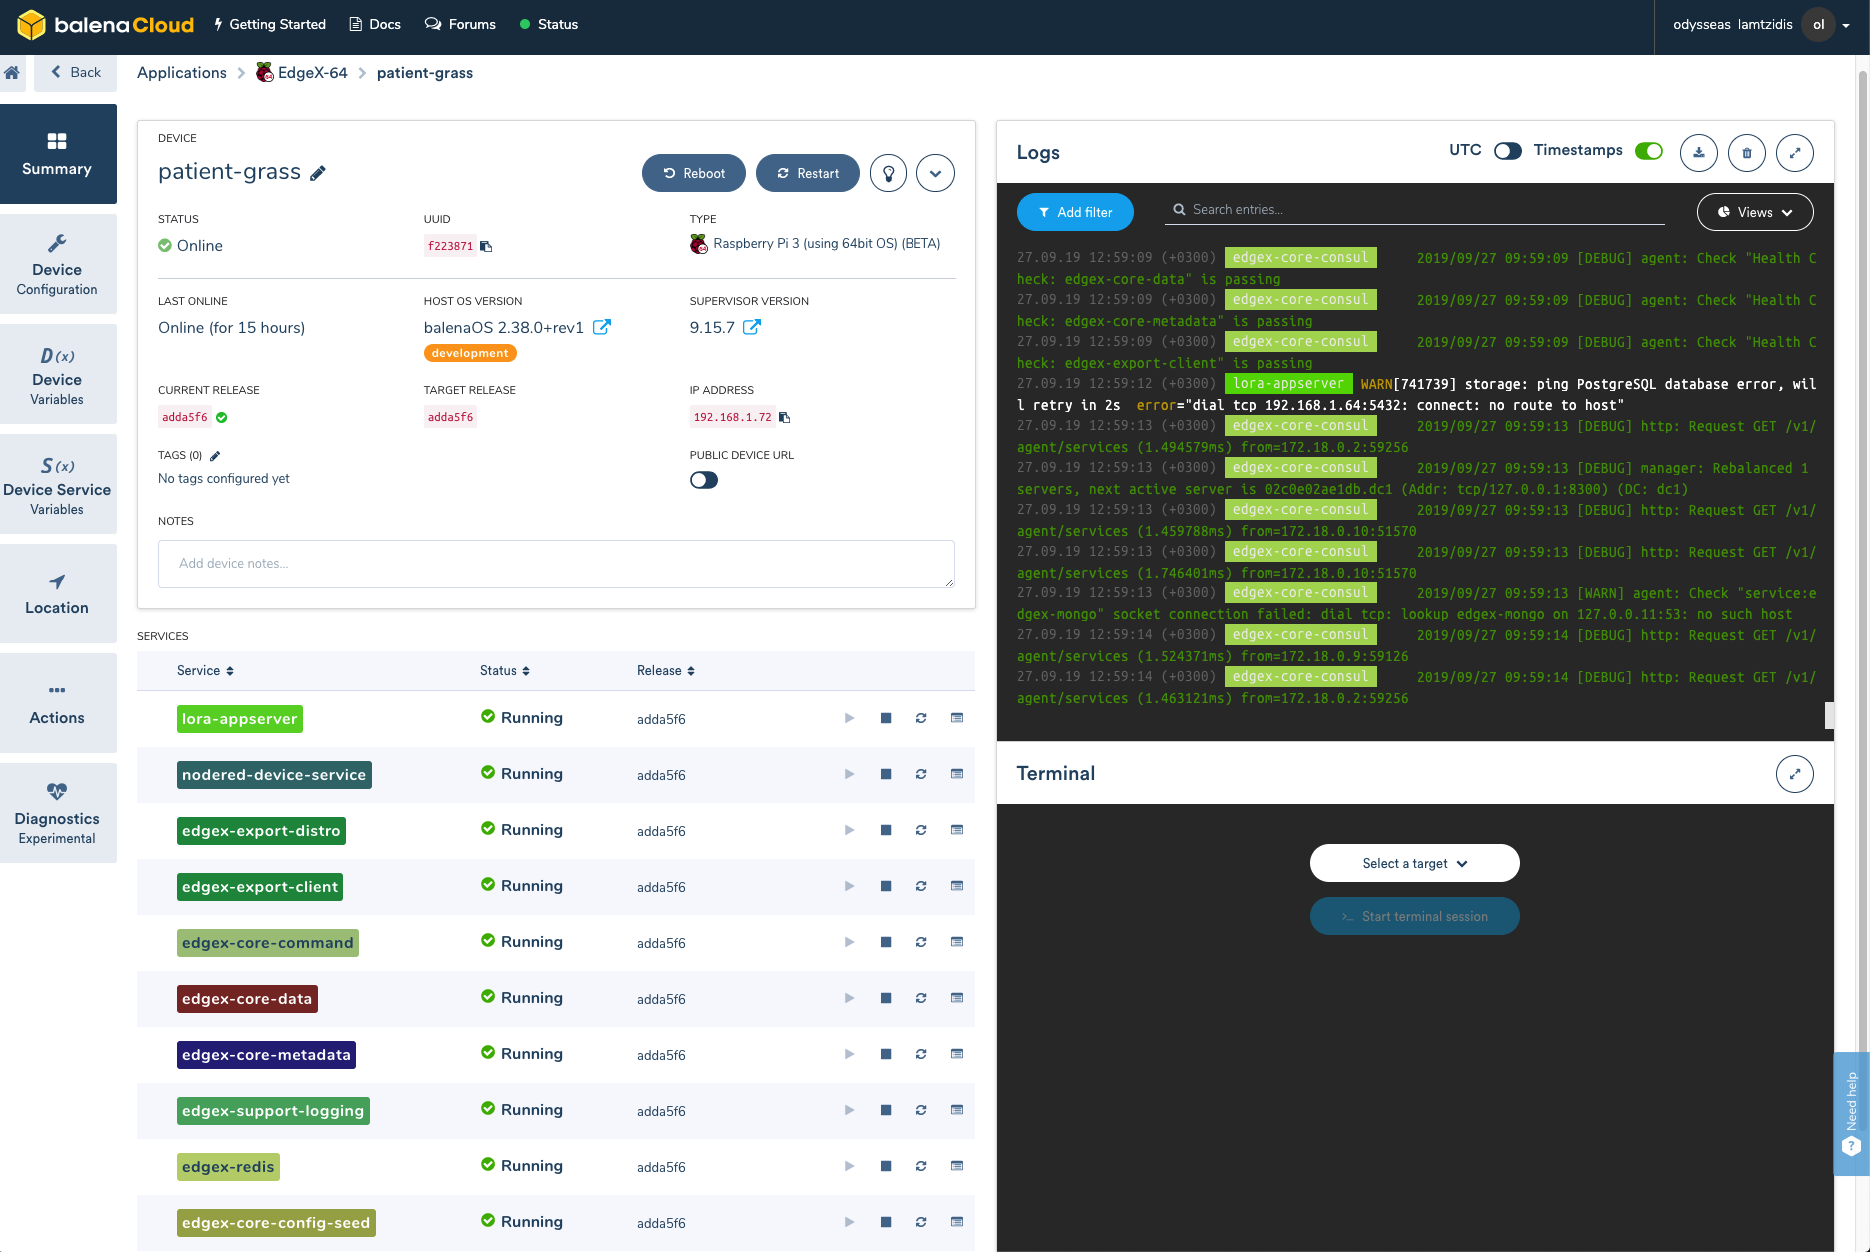
\includegraphics[width=0.9\textwidth]{images/balena_device.png}
    \caption{Balena Dashboard: The device view where device-specific information is shown}
    \label{fig:balena_device}
\end{figure}

In balena, devices belong to a certain application, thus each device added to that application will be installed with exactly the same software. Applications are described as a set of containers (1 to n distinct containers) and their relationship and installation are described by docker-compose version 2.1. In practice, balenaEngine supports a subset of the available docker-compose syntax and functionality, while at the same time enriches it with custom fields, relevant to the balena use-case, such as whether the container should have hardware access. 

\subsection{EdgeX Setup}

Having installed balena, the user now needs to populate the device with services. In order to install EdgeX to balena, the user needs to navigate to the developer-scripts repository of the EdgeX organisation at Github\cite{edgex-github} and find the proper docker-compose that is built for the intended architecture (aarch64-ARM64).

The user might observe that the images dictated in the docker-compose do not mention a specific architecture in their name. This is due to the fact that docker.hub, the image registry from where these images are pulled from, supports images with multiple architectures. Depending on the architecture on which the docker engine runs, docker engine is able to request the correct image from the registry, thus this part is abstracted from the developer.

The version that we integrated into the implementation is 1.0.1 “Edinburgh” which is in fact the first release of EdgeX Foundry. We opted to use the EdgeX docker-compose flavour that supports the Redis\cite{redis} in-memory datastore as storage solution, instead of the Mongo database. This is important for performance issues, as Mongo\cite{mongo} memory requirements rendered the Raspberry pi unusable.

Redis is an extremely efficient in-memory database, which periodically creates a file backup in order to save the state in case of an unexpected shutdown. At this point, it’s important to note that such a solution is sub-optimal for Edge Nodes that need to store the aggregated data over long periods of time, as the data-store’s footprint on the memory will grow substantially. As such, a periodic reset of the data-store is needed; this could be time-based (e.g everyday, at 12:00am) or event-based (e.g if data is pushed to the Filecoin network, then delete).

Regarding our EdgeX installation, we opted to install only a subset of the available EdgeX Foundry services in order to keep the platform’s memory footprint as minimal as possible without sacrificing any of the needed functionality. We proceed to define these services into the docker-compose, following the structure as it is defined in the Edinburgh release docker-compose.

\bigskip
\noindent
\textbf{Installed EdgeX modules:}
\textit{\begin{itemize}
    \item volume
    \item edgex-core-consul
    \item edgex-core-data
    \item edgex-core-metadata
    \item edgex-core-config-seed
    \item edgex-core-command
    \item edgex-Redis
    \item edgex-support-logging
\end{itemize}
}
The final version of the docker-compose can be found at the balena folder of the repository. We note that , in order to remove unnecessary complexity, we have changed the name of the services and removed any networking setting, enforcing thus the services to communicate over the default Docker bridge.

The change of the name of the services is due to the fact that EdgeX services are hard-coded to communicate using the host-names, indicated in the official docker-compose, thus we are enforced to change the services name to the original host-names so they are discoverable one from another. At this point, it is apparent to the reader that containers over the same bridge can communicate using either the container names as host-names or by enforcing another host-name through the appropriate attribute in the docker-compose.

\subsection{Installing EdgeX on Raspberry pi using balena}
To install EdgeX, the user needs to open terminal and:
\begin{enumerate}
    \item \texttt{cd} into working directory
    \item run \texttt{sudo balena login}
    \item run \texttt{sudo balena push <application name>} \textit{\#application name was give during the application creation in previous steps}

\end{enumerate}
The source files will be uploaded into balena servers to build the images, either building them from the source as specified in a Dockerfile, or pulling them from a registry. The EdgeX application will be shipped as soon as the build is ready. The supervisor will then proceed to download the application, pause any running containers and perform the install of updated and new containers and the removal of containers that are no longer defined in the docker-compose file. Finally, the supervisor kick-starts the services according to the dependencies that are also defined in the docker-compose.

\bigskip
\noindent
\subsubsection{EdgeX Walkthrough}
The key aspect the user needs to get acquainted with in EdgeX is the API resources of each microservice, especially if the user intends to integrate other services to the EdgeX Foundry platform. The user is advised to follow the EdgeX API walkthrough tutorial that can be found in the EdgeX documents\cite{edgex-api}, as also review the API docs for each microservice. In this process and for debugging purposes, the use of Postman is advised, as it greatly facilitates it. On top of that, EdgeX offers a set of API tests that can be imported to Postman and function as templates for further experimentation; they can be found in the \textit{developer scripts} Github Repository mentioned earlier.

\subsection{Filecoin setup}

\subsubsection{Client (Storage Consumer) setup} \label{sub:filecoin-client-setup}

In order to interact with the Filecoin network, a user needs to setup a Filecoin Node by following the in-depth walkthrough tutorial \cite{filecoin-walkthrough}.

Filecoin currently is available only for linux and macOS as it is still in alpha version, demanding at the same time, considerable computer resources to run efficiently as the various components are still in development and little optimisation has been made. It is recommended to have at-least a 4 core x86 modern processor and 8GB of RAM, moreover the user should expect to leave the computern running for an extended period of time (in order to synchronise with the network), so the use of a cloud Linux server would be ideal. 

Finally, note that as the go-Filecoin daemon will run in the foreground, it will block the terminal session (or ssh), continuously outputting logging information from the Filecoin node, as shown in Figure \ref{fig:filecoin_terminal}. For this reason, the use of the \texttt{screen} application is advised. \texttt{screen} enables to create virtual terminal sessions from which you can attach and detach, all from one actual terminal session. When detached, the virtual sessions continue to function normally and when attached again, the user can inspect the session history.

\begin{figure}[h]
    \centering
    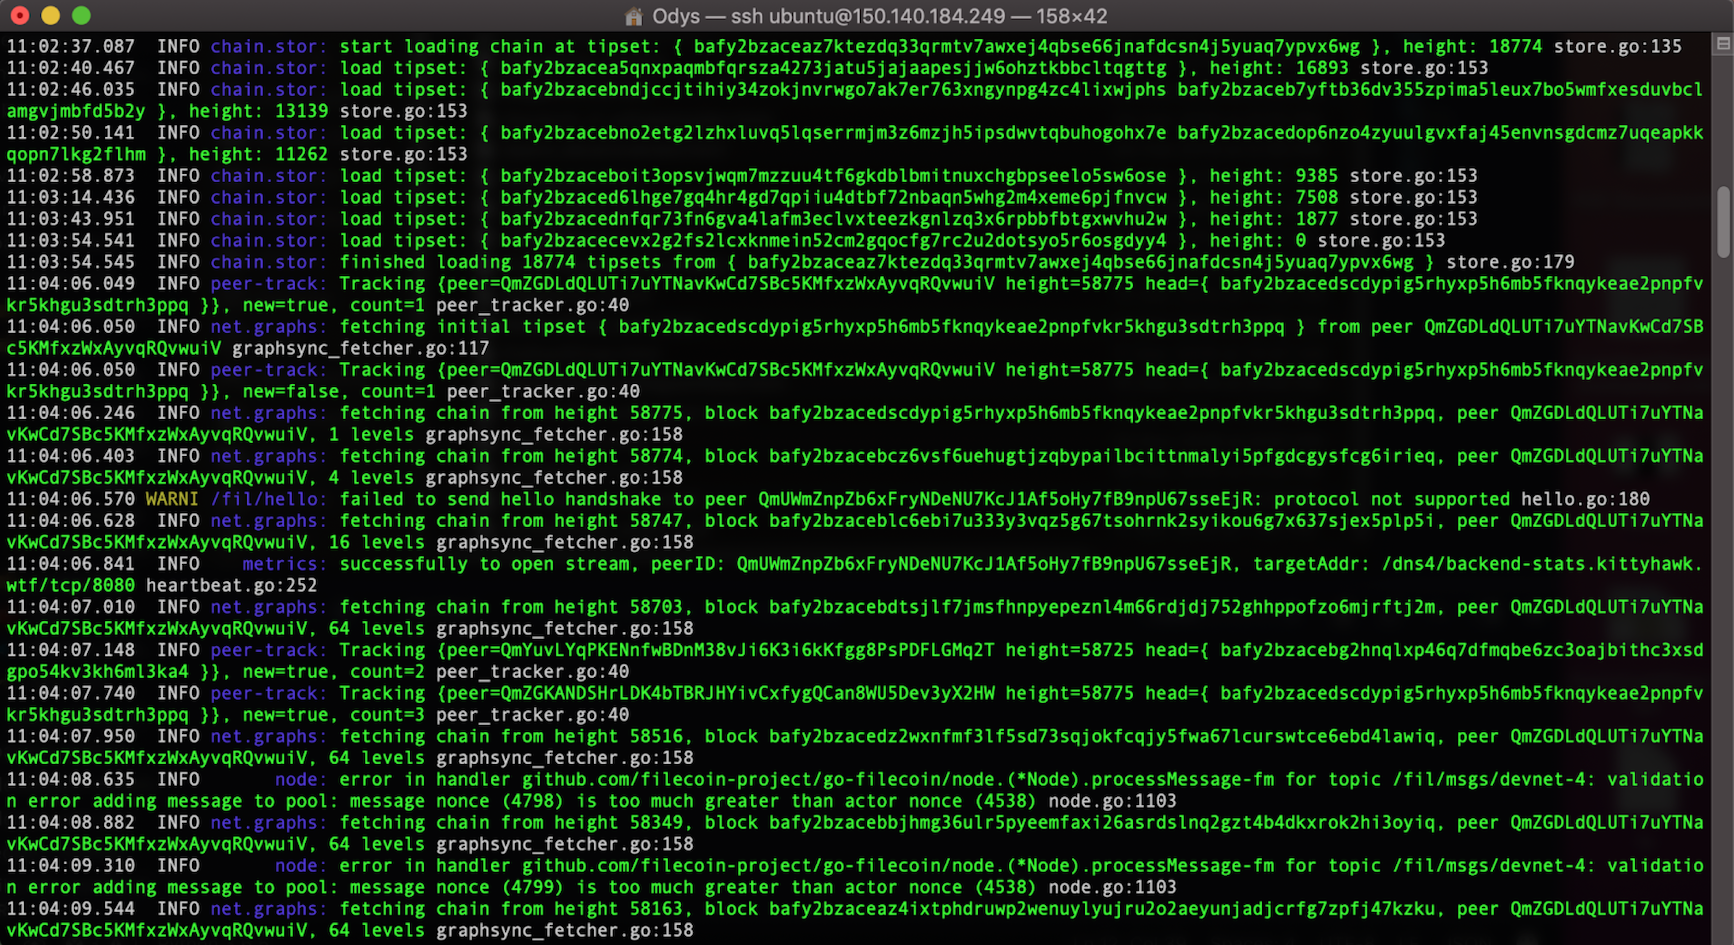
\includegraphics[width=1\textwidth]{images/filecoin_terminal.png}
    \caption{A terminal window outputting STDOUT from go-filecoin daemon}
    \label{fig:filecoin_terminal}
\end{figure}

In order to use the Filecoin network as storage client, the user needs to use the Filecoin faucet and fill the node’s wallet address with Devnet FIL, as outlines in the already referenced walkthrough tutorial.

\subsubsection{Miner (Storage Provider) setup}

In the Filecoin docs, the user can also learn about setting up a filecoin node for mining. We remind the reader that in the Filecoin network, the blockchain miner is the storage provider and mining power is a function of the provided storage and the available storage in the network. When mining, the storage provider gains FIL by providing storage (ask orders) and by verifying and sustaining the integrity and correctness of the blockchain.


\subsubsection{Notes}
We find enlightening to further expand on some parts of the walkthrough.
\begin{enumerate}
    \item \textit{Commit storage?} In the current Filecoin implementation, the miner does not commit a specific amount of storage, but rather it is committed in an ad-hoc basis. The miner sets the price and it automatically accepts any deal from any client.
    \item \textit{Price?} The listed price is in FIL/byte/block. In the blockchain, a new block is mined roughly every 30s, thus in a day (24 hours * 60 minutes * 60 seconds) 2880 new blocks are mined. If the miner wants the price to be valid for a day, he will set a limit of 2880 blocks. Conversely, if a client wants to store 1 byte for 1 day and the price is 1 FIL, then he will pay to the storage provider 2880 FIL.
    \item \textit{gas?} The gas is a term popularised in the ethereum ecosystem. In essence, each time a block is mined, the block miner(s) earn not only the reward in that block, but also the gas given by all the nodes whose transactions are encapsulated into that block. The higher the gas value, the more “valuable” the transaction will be for the prospecting miners, thus it will have a higher priority to be put into the next block over other transactions. (faster confirmation rate).
\end{enumerate}

\section{Lorank8 setup}
Lorank comes pre-installed with certain software but the user will need to enrich it for this implementation. An in-detail guide of how to Quick start with the Lorank8 can be found on Github\cite{Lorank8-manual}, maintained by the company that manufactures and sells Lorank8 itself. A thorough reading of the document is prerequisite to understand the device and start the custom configuration. After following the steps dictated in the Quick Start section of the manual, the user can proceed in configuring the gateway.

\subsection{Configure ssh and install software in Lorank8}
Before continuing, it’s time to introduce an elementary (though highly important) piece of software. SSH, also known as Secure Shell or Secure Socket Shell, is a network protocol that gives users, particularly system administrators, a secure way to access a computer over an unsecured network. SSH also refers to the suite of utilities that implement the SSH protocol. Secure Shell provides strong authentication and encrypted data communications between two computers connected over an open network such as the internet.

In order to ssh into Lorank, the user can either use the local hostname of the device, leveraging the local avahi software that exists or the local IP. In order to connect by using a local IP, we used the program \textit{lanscan} to search for all the devices that exist in the local network and then find the device with hostname “Lorank8”. To use avahi, we simply use “Lorank8.local” in place of the IP. The .local suffix tells avahi to search the network for a device with hostname “Lorank8”.

Now that there is an open ssh connection with Lorank8, it’s time to install the software that will be used (e.g loraserver.io suite). The following commands are executed in order to update the system and install the required software.

\begin{minted}[%
 breaklines,
 mathescape,
 linenos,
 numbersep=5pt,
 frame=single,
 numbersep=5pt,
 xleftmargin=0pt
 ]{bash}
apt-get install update 
apt-get upgrade
apt-get install screen #the same program mentioned in Subsection $\ref{sub:filecoin-client-setup}$
apt-get install htop #a visual upgrade of the top command, used for debugging.
\end{minted}
Then, we proceed to install a MQTT broker (mosquitto), add the LoRaserver repository to the repository lists of the device and install LoRaserver gateway bridge and LoRaserver network server.

\begin{minted}[%
 breaklines,
 mathescape,
 linenos,
 numbersep=5pt,
 frame=single,
 numbersep=5pt,
 xleftmargin=0pt
 ]{bash}
apt-get install mosquitto
sudo apt-key adv --keyserver keyserver.ubuntu.com --recv-keys 1CE2AFD36DBCCA00
sudo echo "deb https://artifacts.loraserver.io/packages/3.x/deb stable main" | \
sudo tee /etc/apt/sources.list.d/LoRaserver.list
sudo apt-get update
sudo apt-get install Redis-server
sudo apt-get install LoRa-gateway-bridge
sudo apt-get install LoRa-LoRaserver

\end{minted}

Finally, LoRaserver network-server requires Postgresql\cite{postgresql} to function. This is challenging since the official support of Postgresql for beaglebone (armv7 architecture / debian 8 “Jessie”) is until version 9.4 but LoRaserver requires version 9.5+. Thus, we will have to use the backports version of Postgresql 9.5 stretch debian.

Backports are re-compiled packages from testing (mostly) and unstable (in a few cases only, e.g. security updates) in a stable environment so that they will run without new libraries (whenever it is possible).

Thankfully, some online research came to fruition\cite{backport}, providing the Lorank8 with the appropriate version of Postgresql.

\bigskip
\noindent
\subsubsection{Configuration of Postgresql}
Having installed Postgresql, it is now required to create a database for LoRaserver to use, so we run the following commands:

\begin{minted}[%
 breaklines,
 mathescape,
 linenos,
 numbersep=5pt,
 frame=single,
 numbersep=5pt,
 xleftmargin=0pt
 ]{bash}
sudo -u postgres psql
create role LoRaserver_ns with login password 'dbpassword';

-- create the LoRaserver_ns database
create database LoRaserver_ns with owner LoRaserver_ns;

-- exit the prompt
\q
\end{minted}

\noindent
Finally, if the following command run successfully, the setup is completed.

\begin{minted}[
 breaklines,
 mathescape,
 linenos,
 numbersep=5pt,
 frame=single,
 numbersep=5pt,
 xleftmargin=0pt
 ]{bash}
psql -h localhost -U LoRaserver_ns -W LoRaserver_ns
\end{minted}


\subsection{Lorank8 Configuration}
Having installed the necessery software, it is required to configure the gateway. The working directory is the root directory and the configuration files are available on Github.

Firstly, we configure \textit{global\_conf.json} that can be found in the Lorank8v1 directory, the configuration rests unchanged except for the server output, where we change the default TTN to localhost, \textit{port 1700}. In other words, we instruct the packet forwarder to output the UDP packets to the LoRaserver gateway bridge. We restart Lorank service using the following command: \texttt{systemctl restart Lorank.service}. Finally, the user should note down the gateway ID found in the \textit{local\_conf.json }in the same directory, it will be used later in the implementation.

To configure the gateway bridge and LoRaserver, we create the appropriate \textit{TOML} configuration files in our working directory, as per the LoRaserver documents instructions. We opt to have the configuration in the working directory as we will run the services in foreground using \texttt{screen}, so as to monitor logging information and change configuration in a breeze. Configurations are left to default.

\subsection{Start the Lorank8 gateway services}

After establishing an active \texttt{ssh} connection with Lorank, we run \texttt{htop} to overview the running processes, it is pertinent to close any browser connection to Lorank and kill the \textit{node.js} processes (the web server) as we won’t be using the web interface and it can save considerable resources in respect to cpu and memory.

Moreover, the user needs to ensure that Redis and Postgresql run on the device by running the following commands:

\begin{minted}[%
 breaklines,
 mathescape,
 linenos,
 numbersep=5pt,
 frame=single,
 numbersep=5pt,
 xleftmargin=0pt
 ]{bash}
sudo systemctl start Redis-server
sudo systemctl start Postgresql
\end{minted}

The user then proceeds to start 1) \texttt{LoRaserver} gateway bridge, 2) \texttt{LoRaserver} and 3) \texttt{mosquitto} server on 3 distinct \texttt{screen} sessions, by starting a \texttt{screen} session, then running one of the following commands: \texttt{LoRaserver}, \texttt{LoRaserver-gateway-bridge}, \texttt{mosquitto} and then detaching from the \texttt{screen}. 

It is important to run the commands from the working directory so as they use the configuration that is saved in the same directory, otherwise the processes will use the default ones that can be found in the \texttt{/etc/} directory.

Lorank is now ready to be used with the rest of the implementation. Each packet that the concentrator receives, is forwarded to gateway-bridge which in turn converts it into an MQTT message that is picked by the network-server and finally will be routed to the appropriate application server.

\subsection{Arduino LoRa mote setup}

Regarding the LoRa sensor (mote), it uses \acrfull{abp}, where the Device Address and Session keys are pre-configured (unlike OTAA, where a DevEUI and application key is pre-configured, while the DevAddr and session keys are assigned/generated in the over-the-air-activation procedure). This means that the application server will be able to read any reading coming from a mote that has a the specific network key and application key combination. The implementation would also work with an OTAA device, but we chose ABP for simplicity.

To setup Arduino, we used the default sketch found in the Github of Arduino LMIC \cite{Arduino-lmic} .It’s a project based on the IBM LMIC (LoraMAC-in-C) but modified to run on Arduino. After downloading the sketch and the Arduino IDE, we can flash the sketch in the Arduino and make the proper GPIO connections between the shield and the Arduino as stated in the draggino docs\cite{dragino}. As soon as the Arduino is connected to power( either USB or wall-wart), it will start broadcasting to all gateways in a radius of several kilometers. The payload of the Mote is only decryptable by using the combination of the two keys mentioned before, these keys are only known to our Iot Edge device.

\section{Device Service Component}
The device-services function is to integrate a LoRa device to the EdgeX platform. In essence, the device service can be seen as a platform with a south and north side. The south side connects to the LoRa infrastructure of the edge device (network server) while the north side propagates the data it received from the south to the EdgeX infrastructure. Figure \ref{fig:device_service} illustrates the high level architecture of the device service in a highly simplified diagram that focuses on the device service.

Thus, one component is responsible for managing the LoRa device and LoRa infrastructure and the other is responsible for handling EdgeX. Thus, the node-RED service must:
\begin{enumerate}
    \item Interface with 2 different APIs which implement different specifications and semantics
    \item Expose 2 different APIs that follow different specifications and semantics

\end{enumerate}

\begin{figure}[h]
    \centering
    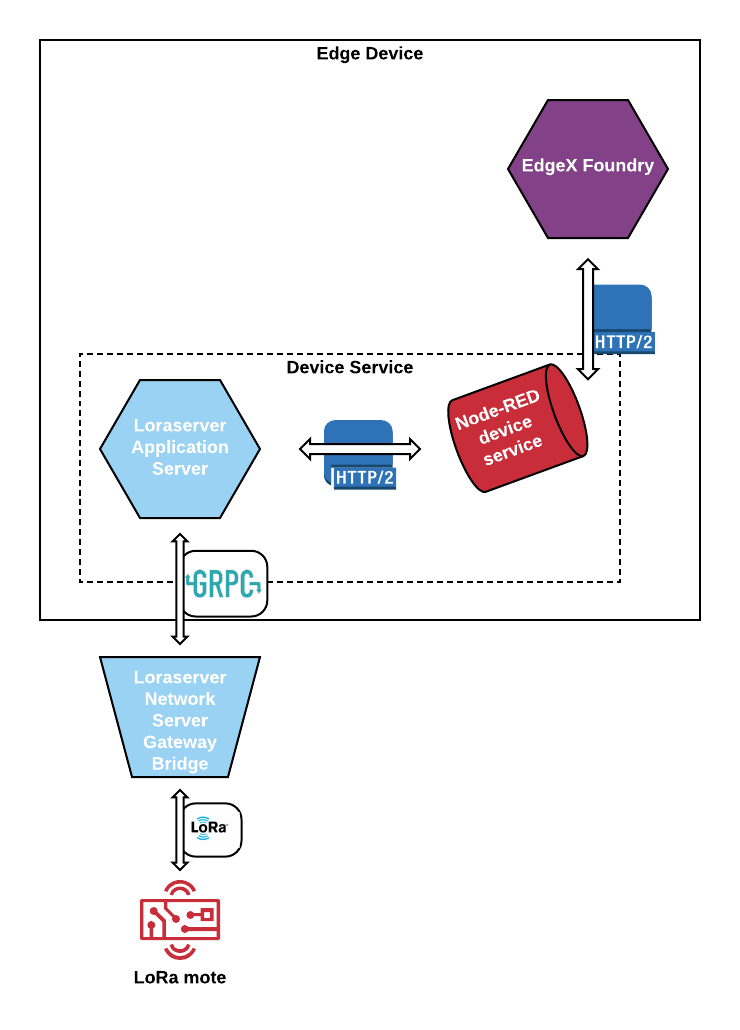
\includegraphics[width=0.7\textwidth]{images/dev_serv_arch.png}
    \caption{High level overview of the Device Service architecture showcasing the main components and their intercommunication protocols}
    \label{fig:device_service}
\end{figure}

The development of the edge service could follow two distincts routes. We could either use the go SDK of the EdgeX, which would serve as boilerplate for the EdgeX component, while we integrate the LoRa part or we could follow the specifications with a custom-tailored solution of our choice. We followed option 2 and instead of using the device service SDK\cite{device-service-sdk}, due to lack of experience with Golang, we opted to-partially-implement the EdgeX device service specification \cite{device-service-spec} in Node-RED.

This is due to the fact that what we needed was a middleware piece of software, that would expose 2 different APIs, one to the LoRa side and one to the EdgeX side. Node-RED is extremely streamlined for the creation of simple API based services, thus the device-service consists of a Node-RED microservice and a LoRaserver-app-server microservice. 

\subsection{Lora application Server}
loraserver.io offers already built images of the platforms, but it is unfortunate that the provided architectures do not include aarch64. Thus, we had to build the container with the application inside. Due to incompatible libraries with the architecture, it was impossible to build the application from source with Dockerfile, thus an intermediate solution was given. The Dockerfile would simply download the binary using \texttt{apt-get install} and then run it in a Alpine Linux BaseOS. Though our approach is not optimal, it is functional and adequate for the proof of concept. 


\subsubsection{Important Note}
A simplification that was made is the existence of the required Redis \& Postgresql server. In lieu of installing new instances in the Raspberry, it was opted that the app server will use the Redis and Postgresql servers that were already installed in Lorank8. It was necessary as Raspberry would not be able to support the load of all the services that we wanted to run.

This is important as the device-service, per the architectural demands, must be fully stateless and without dependencies. Thus, it would require that a total of 4 microservices (i.e node-red, LoRa app server, Postgresql, Redis) would be migrated so as the service provider to function as expected. In our scenario, there is a migration of 2 services (i.e node-red, app-server), while the other two are omitted. 

\subsection{Node-RED setup}
The best deployment method is to develop the node-RED locally and then extract the flow to the Node-RED runtime on the production machine. To install Node-RED locally, the user will use docker and follow the detailed documentation\cite{nodered-docker} provided by the development team. Using the Node-RED graphic editor, the user can start creating flows. Flows are different parts of the application that run in parallel and can be used to distribute the application logic and increase "code" readability.

The device-service state machine has only two states, the setup state and the normal operation state. We create a flow for each state for ease of use. When Node-RED service starts, the setup flow starts which registers the Node-RED service to both EdgeX and LoRa-app-server. This bootstrap phase is shown in Figures \ref{fig:devserv-boot1} and \ref{fig:devserv-boot2}. After the registration is complete, EdgeX and LoRa-app-server will start making requests to the API resources that we have defined in the second flow shown in Figure \ref{fig:devserv-norm}.

\subsection{Service setup state}
The flow starts with the inject node which outputs the first message as soon as Node-RED starts. Then, we make consecutive calls to the EdgeX platform in order to register the device service, as indicated in the EdgeX API walkthrough tutorial, with a small change: we don’t define a device addressable as indicated in the tutorial, but we define it in when provisioning a new device. To make the consecutive calls, all the HTTP POST requests bodies are defined at the start of the flow and saved as flow variables. Then, before each HTTP request node, we set the \textit{msg.url} and \textit{msg.payload} to the appropriate values. The url depends on the EdgeX service that the request is intended while the payload depends on the registration step. The reader is invited to research our github and see the structure of these payloads, we choose not to analyse further as they are use-case dependent. 

The same methodology is followed for the LoRa-App-Server registration as well, as shown in Figure \ref{fig:devserv-boot2}. The required steps to connect a sensor were found in the loraserver.io docs, but instead of the web interface, the RESTful API was used. Moreover, an HTTP integration is defined so that each time LoRa-app-server receives a reading, it is forwarded to a specific resource. This resource is in fact the Node-RED service that receives the data (south-side) and then makes an HTTP request to EdgeX (north-side). The network keys that were defined during the ABP setup of the Arduino mote are used in order for the application server to be able to decrypt the payloads that are received in the gateway.

\subsection{Service normal operation state}
During normal operation, the service has 5 active API HTTP resources, 4 are used by the EdgeX services and are defined in the EdgeX SDK specifications and one that is used by the LoRa-app-server to forward the LoRa mote readings. Currently the device service offers only one command to the EdgeX platform and the user, but it is possible to implement the whole SDK specification, offering any number of available commands.

\subsection{Containerization}
The containerization of the Node-RED service was based on the reference Dockerfile provided by the developers of the project\cite{nodered-docker}. What we have added is the placement of the \textit{flows.json}, \textit{package.json }and \textit{settings.json} inside the container so as 1) Node-RED loads our flows; 2) add a runtime argument to Node.js to limit the memory consumed by the process 3) configure Node-RED runtime for the implementation (e.g deactivate the GUI editor to reduce memory footprint). The placement of files inside the container is done at build time using the Dockerfile \texttt{}{COPY} command.

\bigskip \noindent
Finally, we comment on some fields of the configuration file of the Node-RED service:
\begin{itemize}
    \item \textbf{Flowfile:} filename of the json file with the flows
    \item \textbf{disableEditor:} if it set "\textit{True}", it disables editor to reduce memory footprint
    \item \textbf{contextStorage:} This is crucial as it dictates to Node-RED whether to save the defined variables (flow, global) in-memory or in-memory and in a file. We need the service to retain its status even after restart, thus we select the latter and configure it via contextStorage.
\end{itemize}

\newpage
\begin{sidewaysfigure}
    \centering
    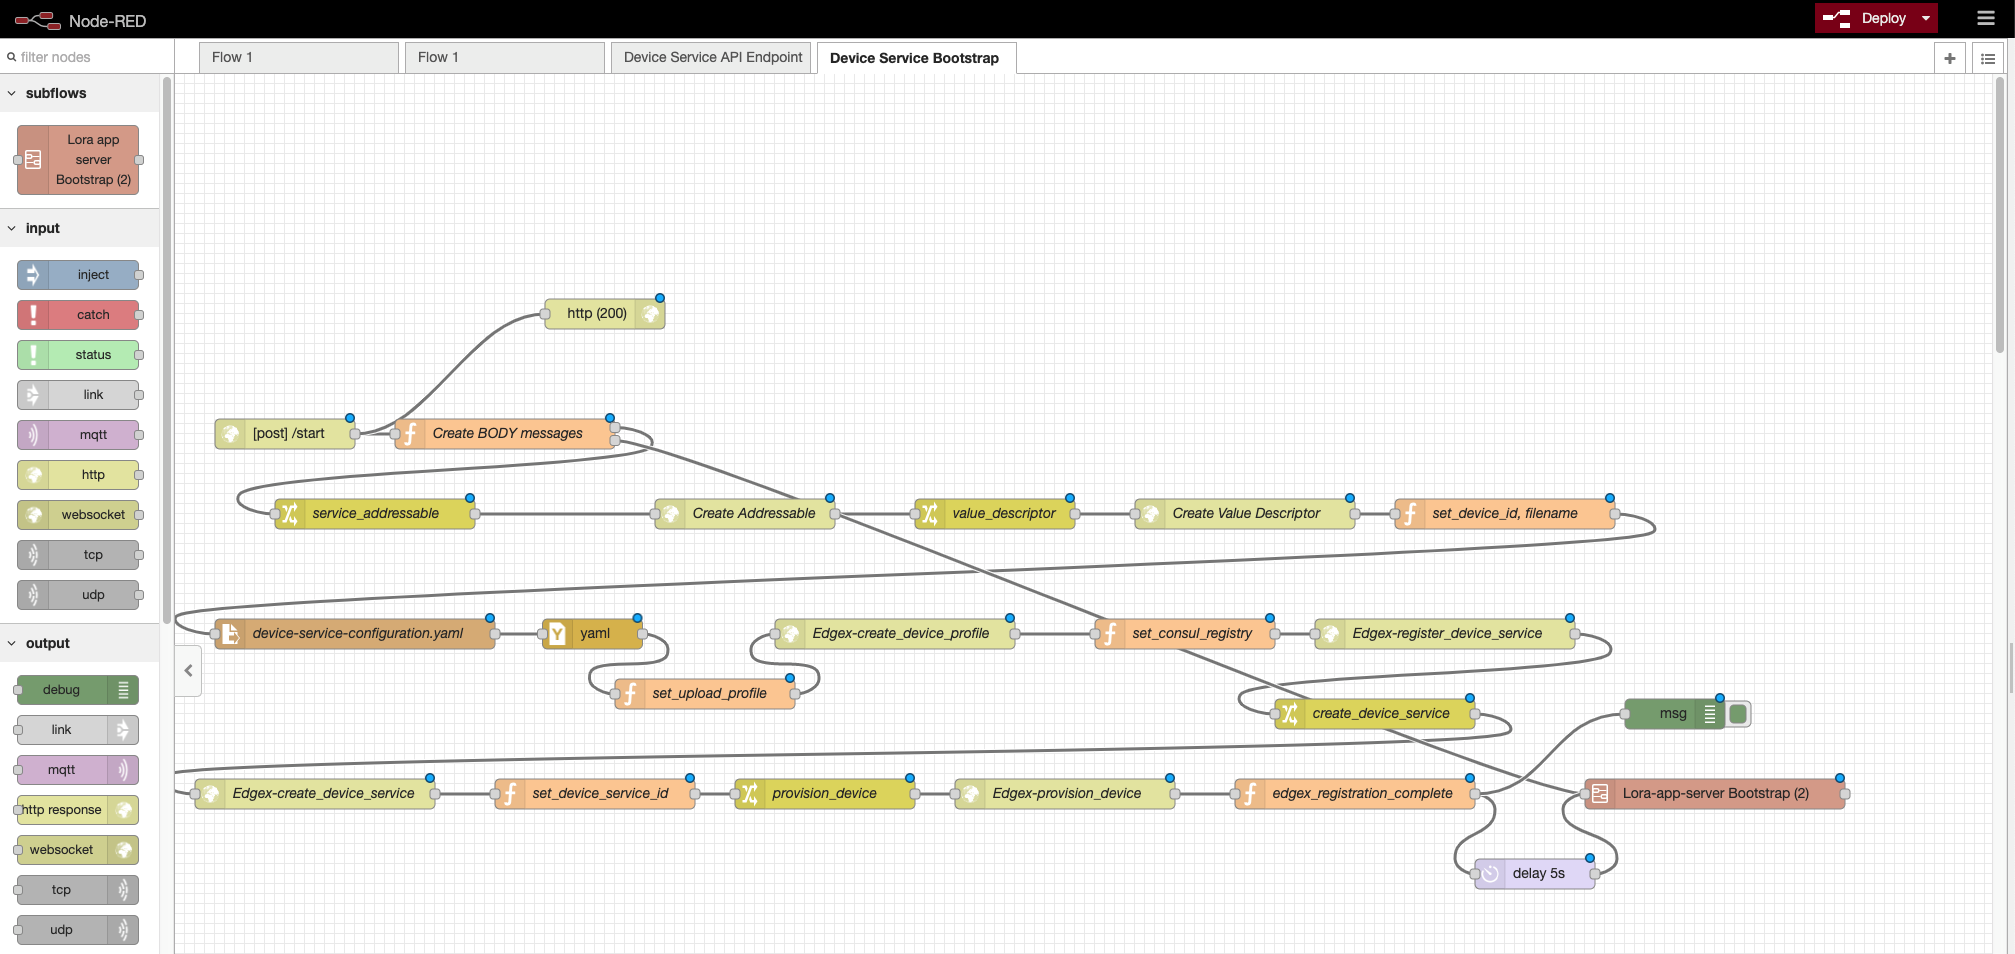
\includegraphics[width=\textwidth]{images/nodered_devserv_boot1.png}
    \caption{The bootstrap flow of the device service Node-RED instance for the EdgeX platform registration}
    \label{fig:devserv-boot1}
\end{sidewaysfigure}

\begin{sidewaysfigure}
    \centering
    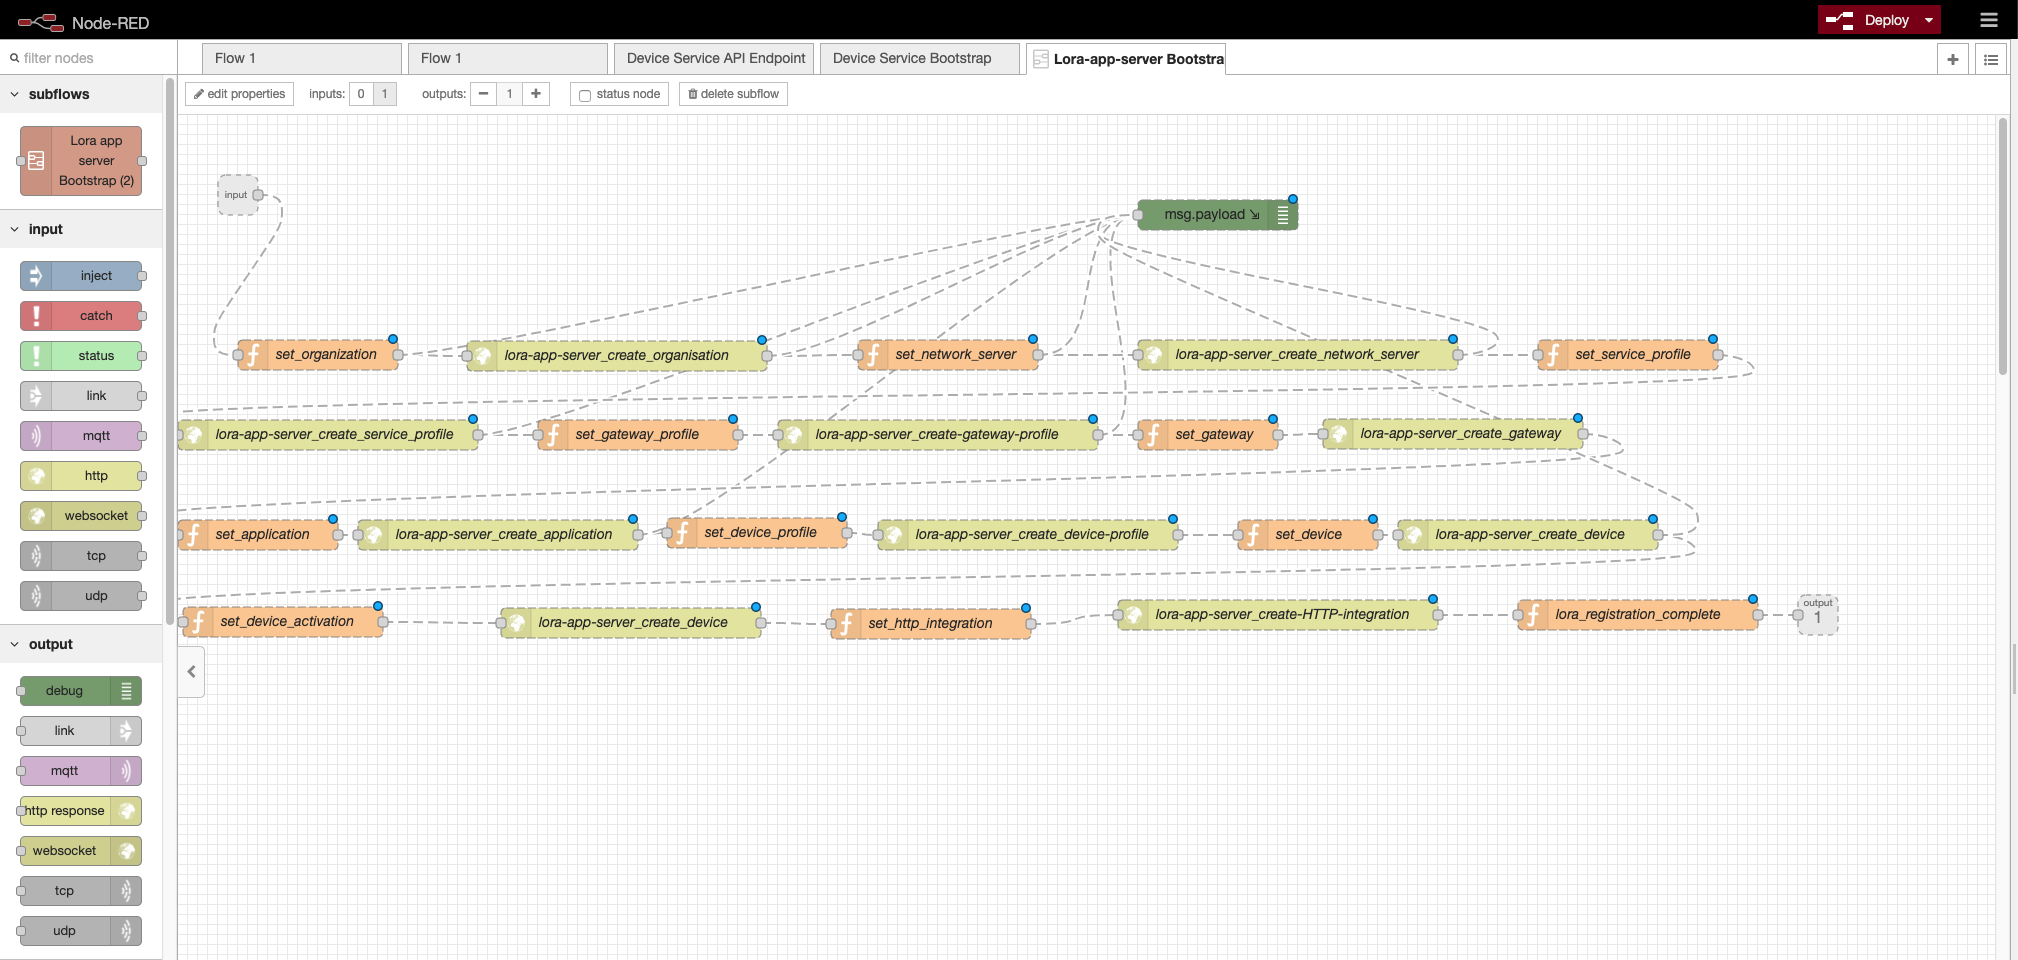
\includegraphics[width=\textwidth]{images/nodered_devserv_boot2.png}
    \caption{The bootstrap flow of the device service Node-RED instance for the LoRaserver application server registration}
    \label{fig:devserv-boot2}
\end{sidewaysfigure}

\begin{sidewaysfigure}
    \centering
    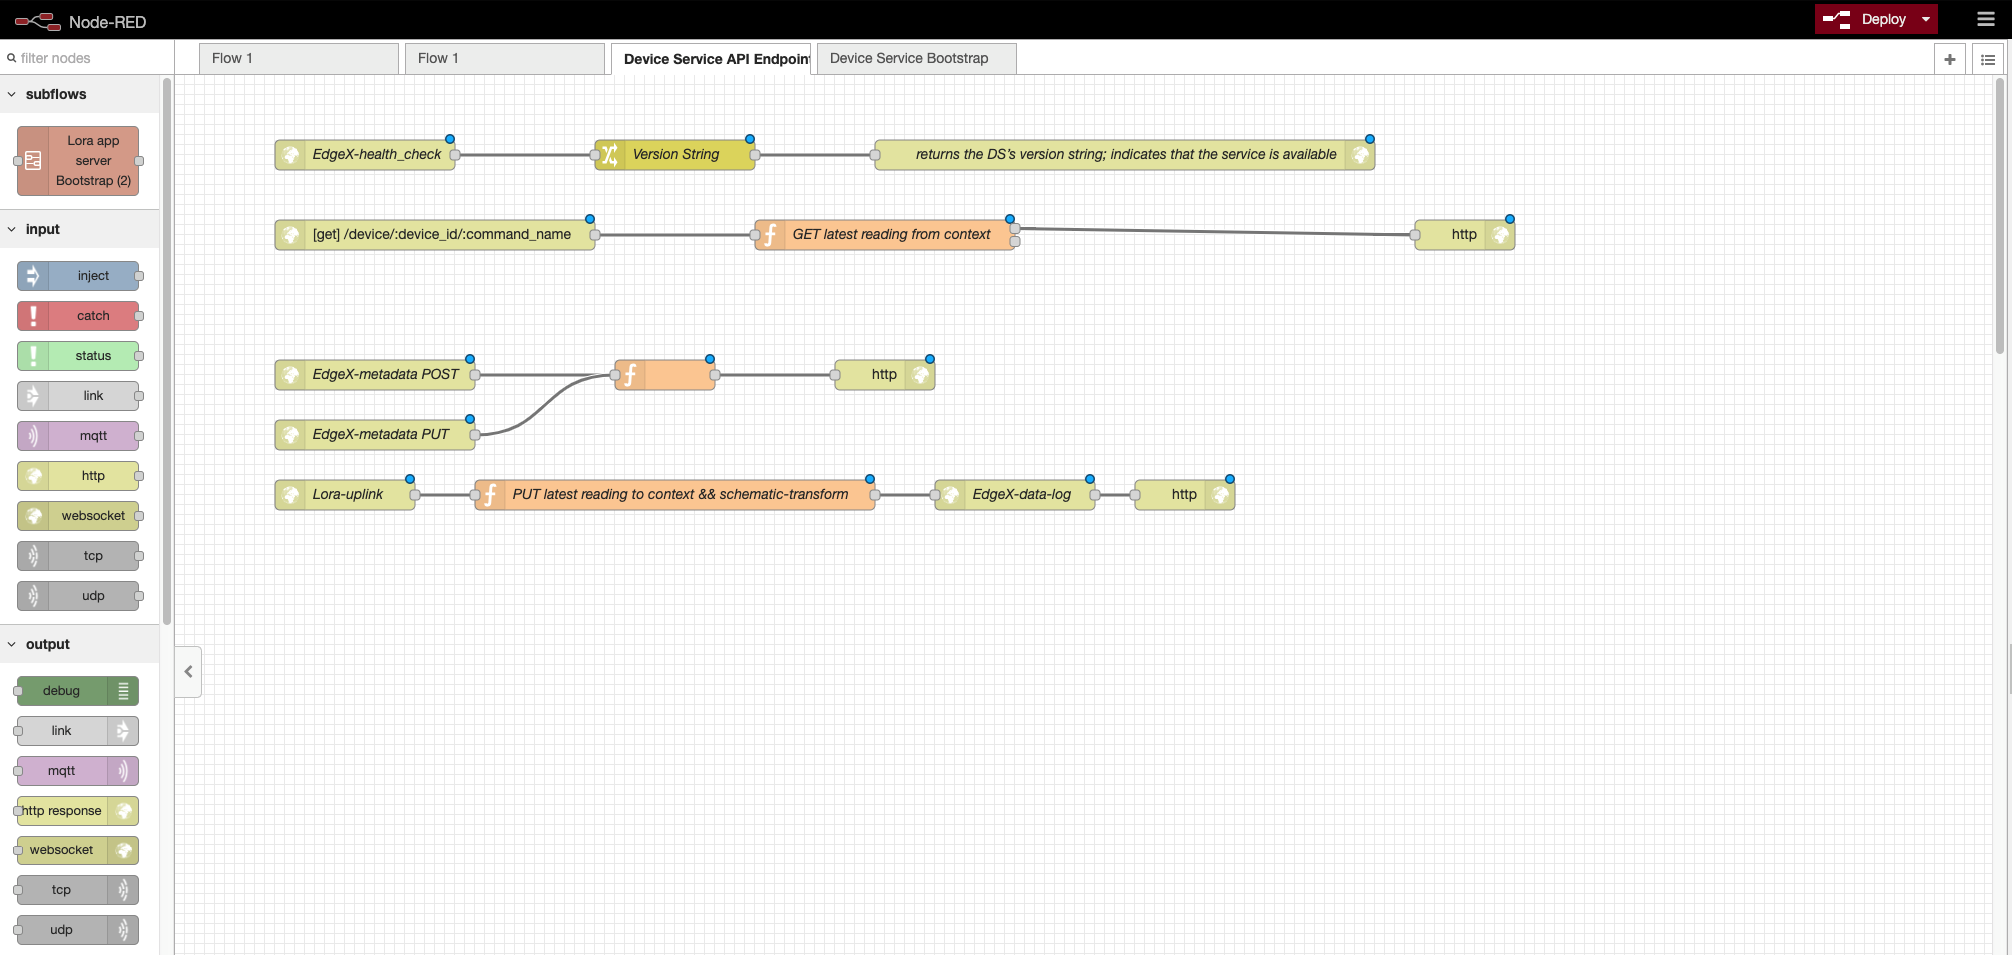
\includegraphics[width=\textwidth]{images/nodered_devserv_api.png}
    \caption{The normal operation flow of the device service is mainly a RESTful API}
    \label{fig:devserv-norm}
\end{sidewaysfigure}

\clearpage

\section{Orchestrator Component}

The orchestrator microservice\footnote{The implementation was partly based on the work of Athanasios Chamalidis, who developed a first implementation and contributed considerably regarding the implemented control of balena supervisor\cite{sakis}.} interfaces and implements multiple functionalities that belong to different services as defined in Architecture Chapter \ref{ch:system-architecture}, namely the \textit{migration service}, the \textit{orchestrator} and \textit{filecoin interface}. It is built in python and based on the flask framework. Flask enabled us to develop quickly while keeping the memory footprint considerably lower than node-red. The service can be logically divided into two parts, the orchestrator and the Filecoin/migration service. Each has its own RESTful API and they are loosely coupled, communicating through their APIs as being two different services. A , rather fancy, component overview can be seen in Figure \ref{fig:orchestrator_component} where we indicate the distinct services that interact in the orchestrator's migration service and the communication protocols.

\begin{figure}[h]
    \centering
    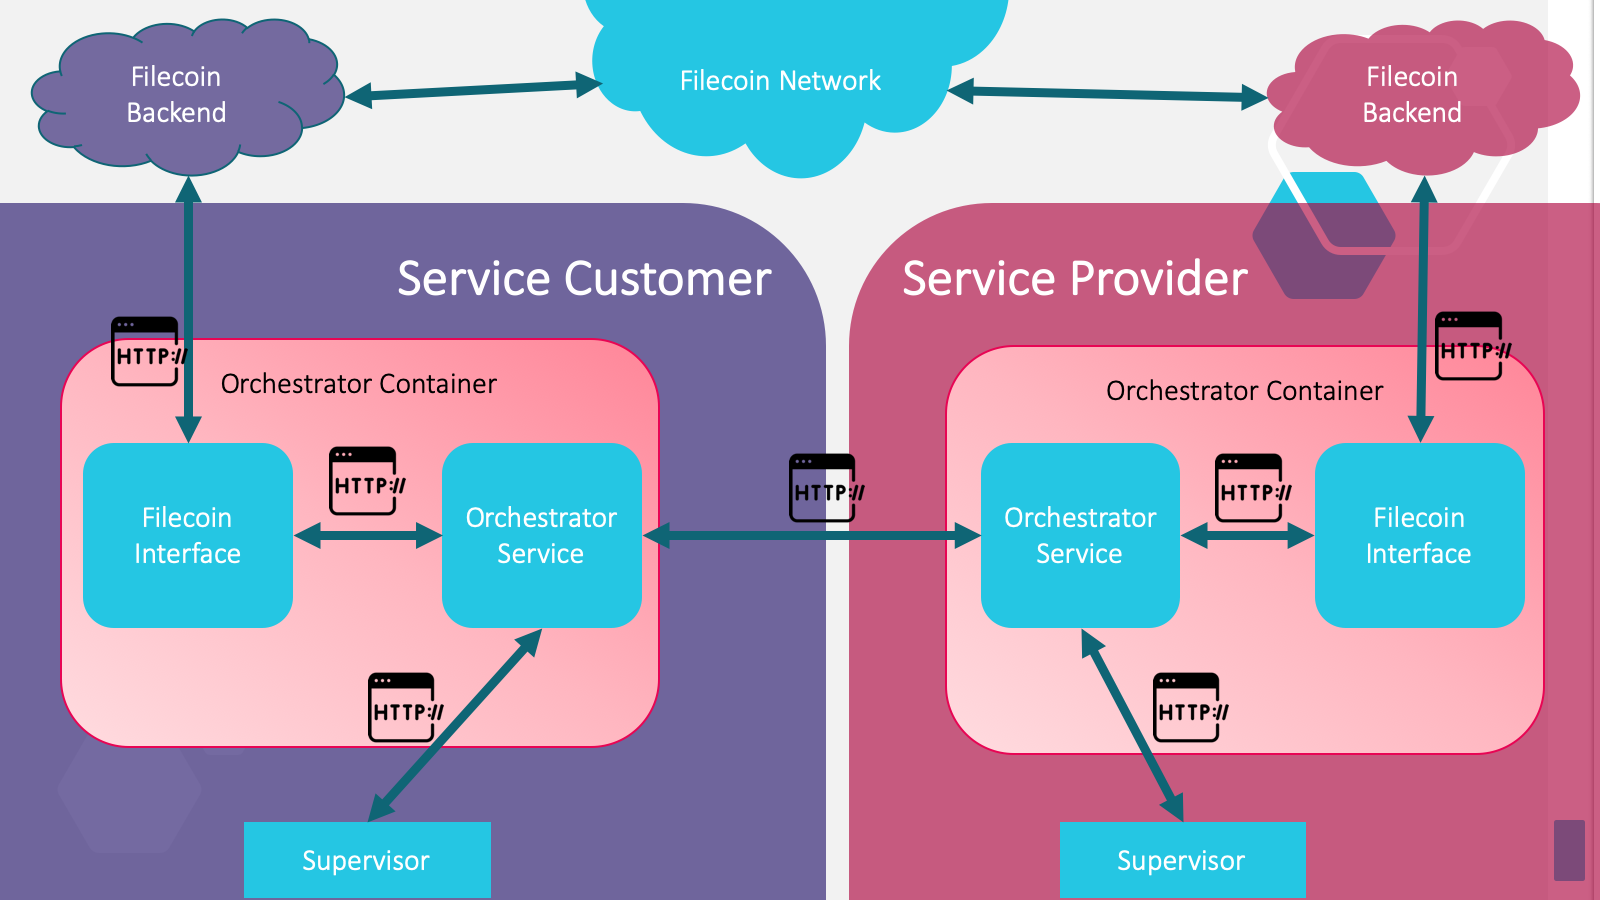
\includegraphics[width=1\textwidth]{images/orchestrator_comp.png}
    \caption{Component overview of the Orchestrator Microservice that is divided into 2 distinct services (orchestrator, filecoin interface)}
    \label{fig:orchestrator_component}
\end{figure}

\subsection{Orchestrator microservice}
\textbf{Functionality:}
\begin{itemize}
    \item Request Filecoin interface to save a container image to the Filecoin DSN
    \item Request Filecoin interface to download a container image from the Filecoin DSN
    \item Load image to balenaEngine
    \item Get balena supervisor state
    \item Set balena supervisor state 
    \item Save \& Load orchestrator from and to a file
    \item Communicate with another orchestrator service and create a service contract
    \item Provide resources for orchestrators inter-communication and Filecoin interface update
\end{itemize}

\subsection{Orchestrator API Resources}

\begin{table}[H]
\centering
\begin{tabular}{|l|l|lll}
\cline{1-2}
\multicolumn{2}{|l|}{{\ul }}                                                                                   &  &  &  \\
\multicolumn{2}{|l|}{\textit{/orchestrator/service\_customer/image/status}}                                    &  &  &  \\ \cline{1-2}
\textbf{{[}GET{]}}  & get the status of all the images of the Edge that are/will be used in a service contract &  &  &  \\ \cline{1-2}
\textbf{{[}POST{]}} & examples:                                                                                &  &  &  \\
                    & \{                                                                                       &  &  &  \\
                    & imageId: 16935cab-2de3-4014-b0f7-3f15eca09bdc16935cab-2de3-4014-b0f7-3,                  &  &  &  \\
                    & imageHash: 7kg8sdf03jdfh9hfsf49h0sdf,                                               &  &  &  \\
                    & status: STORED \# status from [STORED, COMMITED]                                     &  &  &  \\
                    & \}                                                                                       &  &  &  \\ \cline{1-2}
\end{tabular}
\caption{Orchestrator service, REST resource: /orchestrator/service\_customer/image/status}
\end{table} %/orchestrator/service\_customer/image/status
\begin{table}[H] % orchestrator/service\_provider/image/status
\centering
\begin{tabular}{|l|l|lll}
\cline{1-2}
\multicolumn{2}{|l|}{{\ul }}                                                                  &  &  &  \\
\multicolumn{2}{|l|}{\textit{/orchestrator/service\_provider/image/status}}                   &  &  &  \\ \cline{1-2}
\textbf{{[}GET{]}}  & get the status of all images that belong to 3rd parties                 &  &  &  \\ \cline{1-2}
\textbf{{[}POST{]}} & examples:                                                               &  &  &  \\
                    & \{                                                                      &  &  &  \\
                    & imageId: 16935cab-2de3-4014-b0f7-3f15eca09bdc16935cab-2de3-4014-b0f7-3, &  &  &  \\
                    & status: DOWNLOADED                                                      &  &  &  \\
                    & \}                                                                      &  &  &  \\ \cline{1-2}
\end{tabular}
\caption{Orchestrator service, REST resource:  orchestrator/service\_provider/image/status}
\end{table}
\begin{table}[H] %/orchestrator/service\_provider/contract
\begin{tabular}{|l|l|lll}
\cline{1-2}
\multicolumn{2}{|l|}{{\ul }}                                                               &  &  &  \\
\multicolumn{2}{|l|}{\textit{/orchestrator/service\_provider/contract}}                    &  &  &  \\ \cline{1-2}
\textbf{{[}GET{]}}  & get all contracts from the Edge in which it acts as service provider &  &  &  \\ \cline{1-2}
\textbf{{[}POST{]}} & examples:                                                            &  &  &  \\
                    & \{                                                                   &  &  &  \\
                    & edgeId: asdfasdfa,                                                   &  &  &  \\
                    & imageName:asdfadsfas,                                                &  &  &  \\
                    & imageHash:adsfasfda,                                                 &  &  &  \\
                    & config: configFile.json                                               &  &  &  \\
                    & \}                                                                   &  &  &  \\ \cline{1-2}
\end{tabular}
\caption{Orchestrator service, REST resource:  /orchestrator/service\_provider/contract}
\end{table}
\begin{table}[H]
\centering
\begin{tabular}{|l|l|lll}
\cline{1-2}
\multicolumn{2}{|l|}{{\ul }}                                                                                         &  &  &  \\
\multicolumn{2}{|l|}{\textit{/orchestrator/service\_customer/contract/testing}}                                      &  &  &  \\ \cline{1-2}
\textbf{{[}GET{]}}  & get all contracts from the Edge in which it acts as service customer                           &  &  &  \\ \cline{1-2}
\textbf{{[}POST{]}} & examples:                                                                                      &  &  &  \\
                    & \{                                                                                             &  &  &  \\
                    & imageName: LoRa-device-service,                                                                &  &  &  \\
                    & fileName: LoRa-device-service.tar                                                              &  &  &  \\
                    & duration: 7 \#days                                                                             &  &  &  \\
                    & \}                                                                                             &  &  &  \\
                    & \# Resource that is used to start the migration \& contract process, for testing purposes only &  &  &  \\ \cline{1-2}
\end{tabular}
\caption{Orchestrator service, REST resource:  /orchestrator/service\_customer/contract/testing}
\end{table}%/orchestrator/service\_customer/contract/testi
\begin{table}[H] %orchestrator_health
\begin{tabular}{|l|l|lll}
\cline{1-2}
\multicolumn{2}{|l|}{{\ul }}                                         &  &  &  \\
\multicolumn{2}{|l|}{\textit{orchestrator/health}}                   &  &  &  \\ \cline{1-2}
\textbf{{[}GET{]}} & get service status message                      &  &  &  \\
                   & Response:                                       &  &  &  \\
                   & \textit{Status Message: “orchestrator v.0.1.2”} &  &  &  \\ \cline{1-2}
\end{tabular}
\caption{Orchestrator service, REST resource:  /orchestrator/health}
\end{table}

\subsection{Orchestrator's Migration Process}

The orchestrator is built around the Orchestrator class and enables the Edge to function both as a service provider and as a service customer. We give a succinct description of some parts of the code:
\begin{itemize}
    \item \texttt{self.contract\_services\_customer, self.contract\_services\_provider:} data structures (dictionaries) that contain the contracts depending on the role of the orchestrator Edge device.
    \item \texttt{set\_state():} 1) generate device state, by concatenating current state and the new service 2) save orchestrator state in file\footnote{It is necessary because when setting a new state, all unchanged containers restart. We use the volumes file persistency to persist the state of the orchestrator.} 3) set new state.
    \item \texttt{contract\_setup():} updates the contact\_services\_provider dictionary and requests the services image from Filecoin interface
    \item \texttt{check\_contract():} verifies whether the contract activation parameters exist and executes the contract if they are fulfilled. In the current implementation, it is hardcoded to verify the online status of the service customer’s Edge device.
\end{itemize}

The service migration process is initiated manually by the developer by requesting a REST resource and the public URL on where the endpoint of the above resources rest is hardcoded into each Orchestrator service. The process is described in detail by Figures \ref{fig:service_mig_1}, \ref{fig:service_mig_2} where the migration is modeled in a UML sequence diagram. Note that Figure \ref{fig:service_mig_2} is a continuation of Figure \ref{fig:service_mig_1} and in fact the service customer orchestrator entity starts activity in diagram \ref{fig:service_mig_1} and finishes in diagram \ref{fig:service_mig_2}. The implemented process is algorithmically described in Section \ref{st:balena-filecoin}.

\clearpage
\begin{sidewaysfigure}
    \centering
    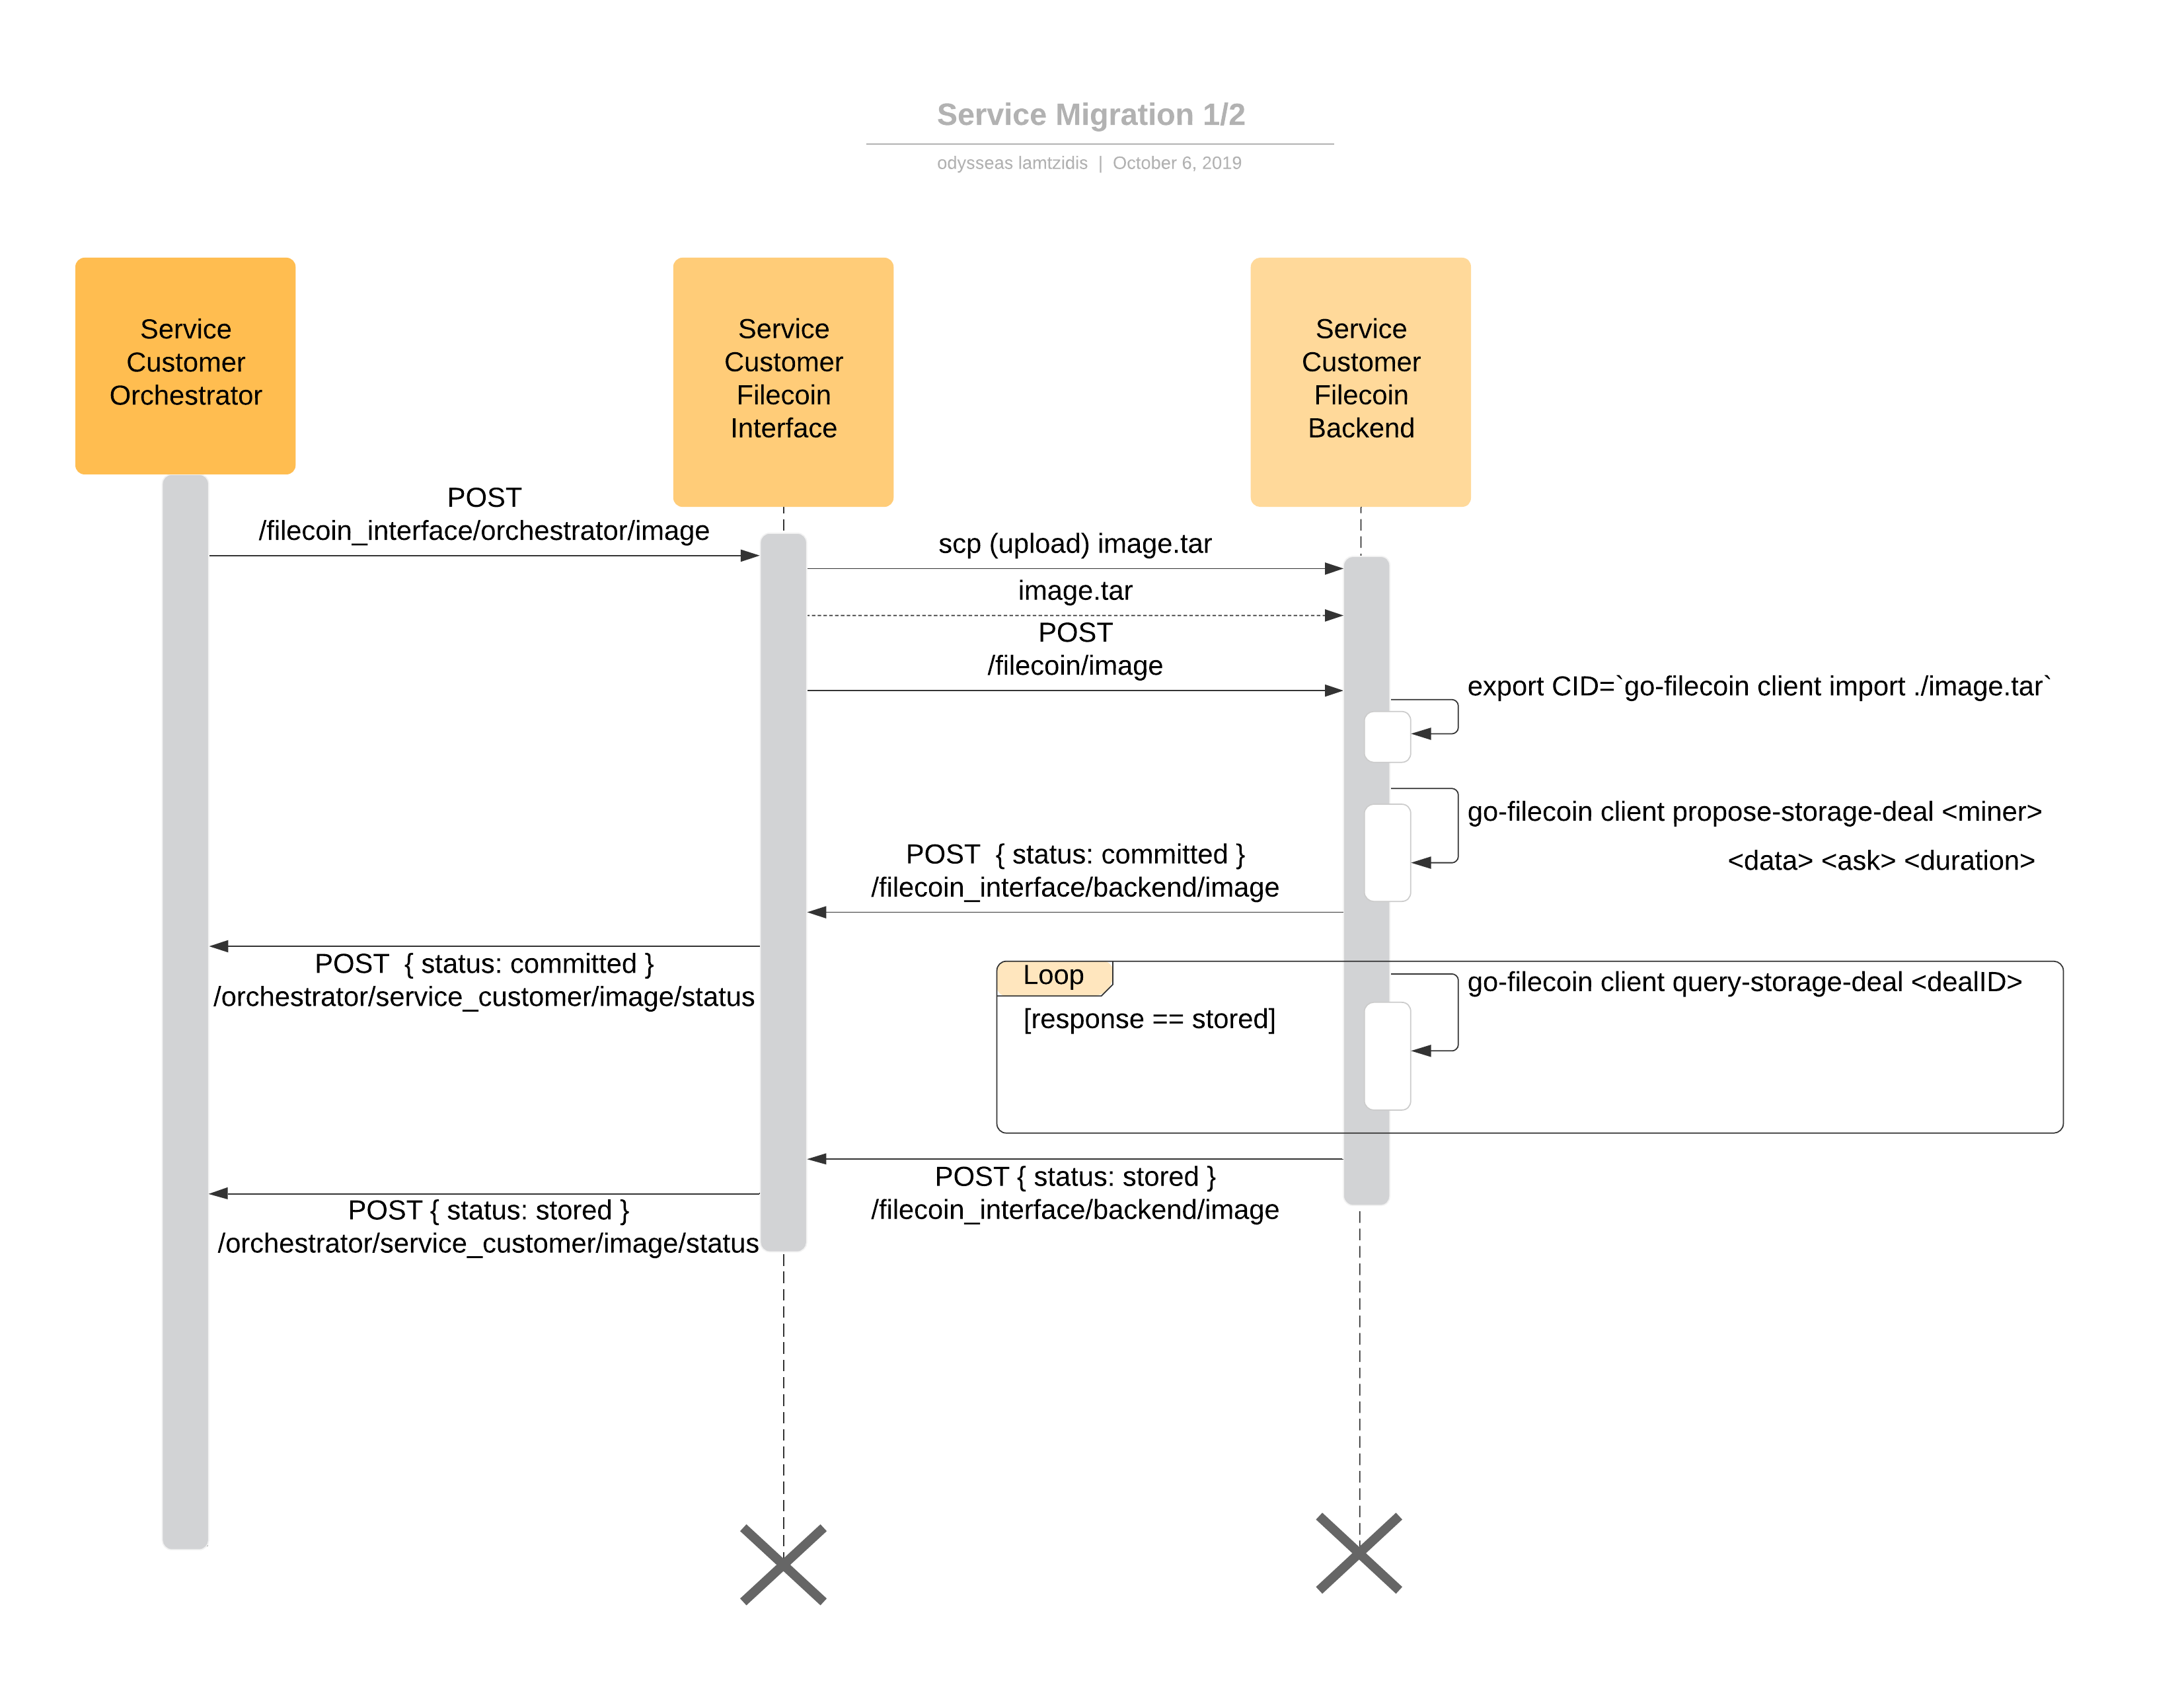
\includegraphics[width=0.9\textwidth]{images/service_mig_1.png}
    \caption{The sequence UML of the migration process, initiated by the Service Customer}
    \label{fig:service_mig_1}
\end{sidewaysfigure}

\begin{sidewaysfigure}
    \centering
    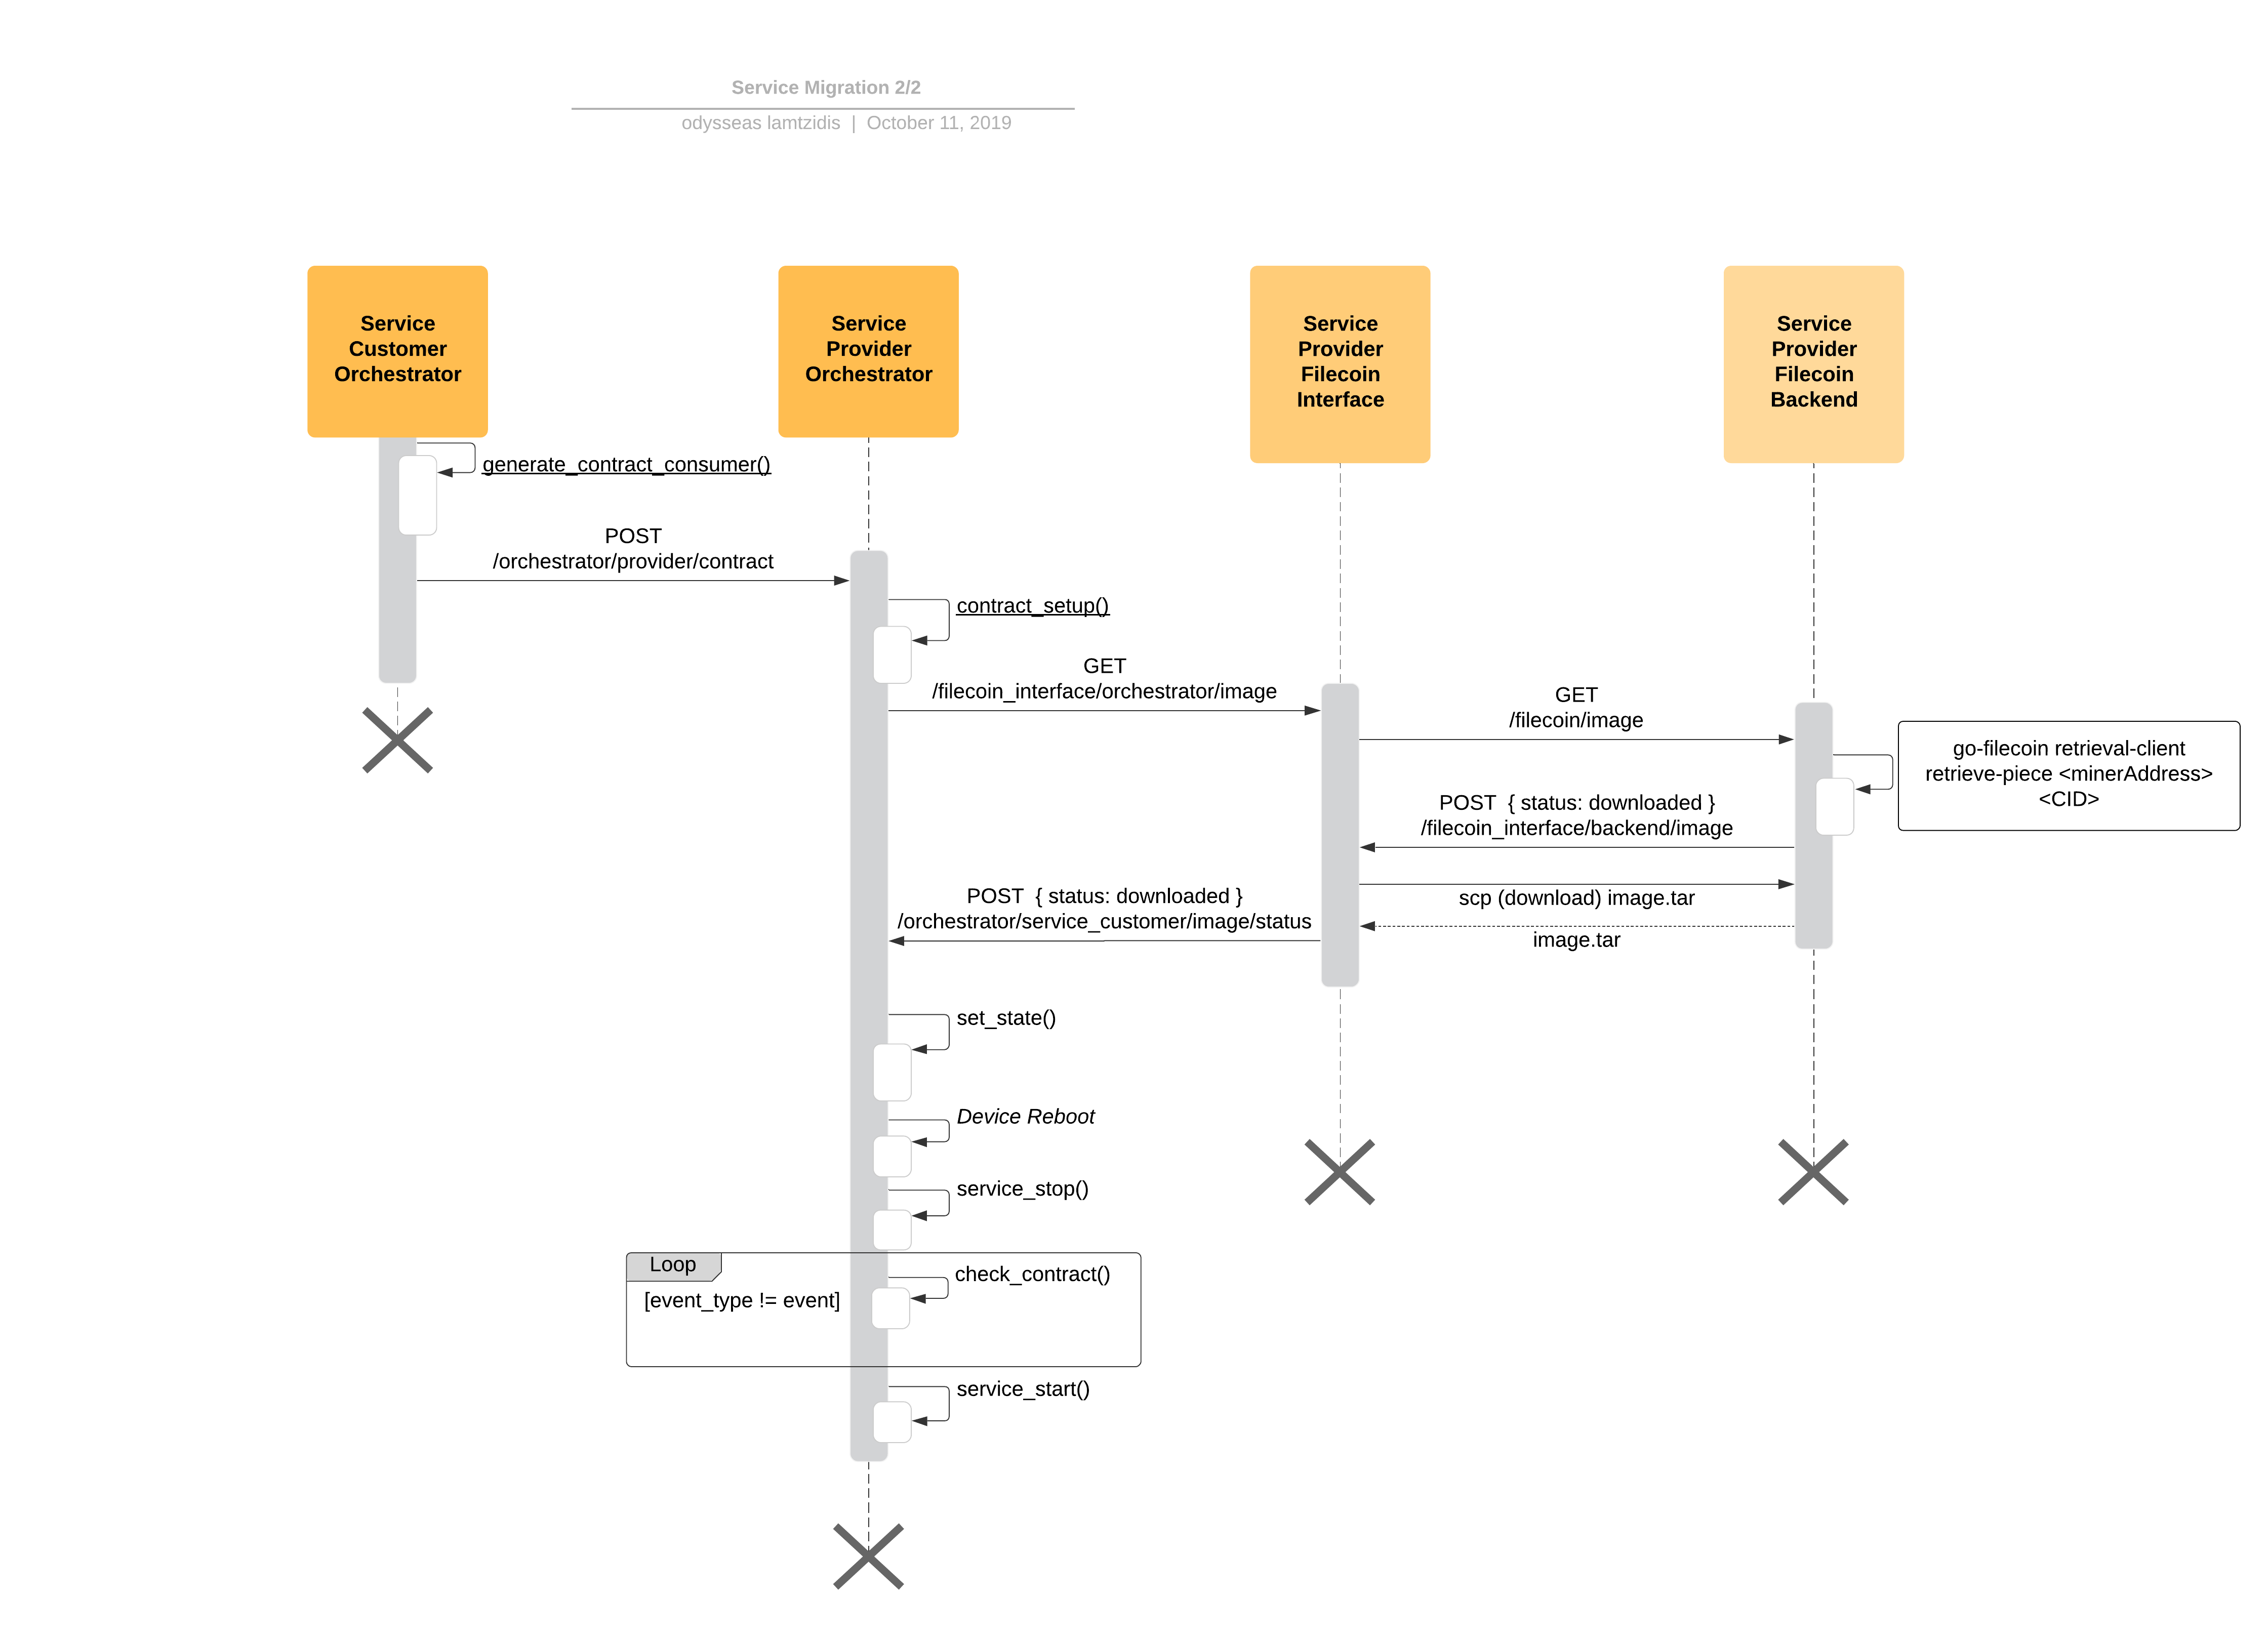
\includegraphics[width=0.9\textwidth]{images/service_mig_2.png}
    \caption{The sequence UML of the migration process (contd.) follow up by service provider}
    \label{fig:service_mig_2}
\end{sidewaysfigure}

\clearpage
\subsection{Filecoin Interface component}

It has a dual role, fulfilling the roles of migration service and the Filecoin network interface. 

As mentioned in Section \ref{st:filecoin}, Filecoin is currently in alpha version and therefore demands high computational resources, rendering it impossible to be run on Raspberry Pi 3. Moreover, the current Official API implementation is incomplete and could possibly have a considerate amount of bugs, decreasing considerably our speed of development. 

Thus, we developed our own Filecoin API, by developing a node-RED application that runs on a cloud Linux server and exposes the Filecoin functionality that we require using 2 RESTful HTTP resources. We call it filecoin interface backend service. The backend service extracts information from the HTTP requests and translates them into Filecoin-CLI commands, functioning exclusively as a wrapper around Filecoin. A screenshot of Node-RED web editor and the aforementioned flow can be seen in Figure \ref{fig:filecoin_backend}.

\noindent
The REST interface of the filecoin interface component is surmised bellow:
% Please add the following required packages to your document preamble:
% \usepackage[normalem]{ulem}
% \useunder{\uline}{\ul}{}
\begin{table}[H]
\centering
\begin{tabular}{|l|l|lll}
\cline{1-2}
\multicolumn{2}{|l|}{{\ul }} &  &  &  \\
\multicolumn{2}{|l|}{\textit{/filecoin\_interface/backend/image}} &  &  &  \\ \cline{1-2}
\textbf{{[}POST{]}} & examples: &  &  &  \\
 & \textit{\{} &  &  &  \\
 & imageid: 16935cab-2de3-4014-b0f7-3f15eca09bdc16935cab-2de3-4014-b0f7-3, &  &  &  \\
 & imageHash: 7kg8sdf03jdfh9hfsf49h0sdf, &  &  &  \\
 & status: STORED  \# status from {[}STORED, COMMITTED, READY2DOWNLOAD{]} &  &  &  \\
 & \} &  &  &  \\ \cline{1-2}
\end{tabular}
\caption{Filecoin Interface service, REST resource: /filecoin\_interface/backend/image }
\end{table} 

\begin{table}[H] %filecoin/orchestrator/image
% \centering
\begin{tabular}{|ll|lll}
\cline{1-2}
\multicolumn{2}{|l|}{{\ul }} &  &  &  \\
\multicolumn{2}{|l|}{\textit{/filecoin\_interface/orchestrator/image}} &  &  &  \\ \cline{1-2}
\multicolumn{1}{|l|}{\textbf{{[}GET{]}}} & \{ &  &  &  \\
\multicolumn{1}{|l|}{} & imageName: LoRa-device-service, &  &  &  \\
\multicolumn{1}{|l|}{} & imageHash: 7kg8sdf03jdfh9hfsf49h0sdf, &  &  &  \\
\multicolumn{1}{|l|}{} & minerAddress: QmfVk1c4Byn5E5He6Sk7Y8NTRNUtfBE7yhJedpDwi94rat &  &  &  \\
\multicolumn{1}{|l|}{}  & \} &  &  &  \\ \cline{1-2}
\multicolumn{1}{|l|}{\textbf{{[}POST{]}}} & \{ &  &  &  \\
\multicolumn{1}{|l|}{} & imageName: LoRa-device-service, &  &  &  \\
\multicolumn{1}{|l|}{} & storageDuration: 7 \#days, &  &  &  \\
\multicolumn{1}{|l|}{} & fileName: LoRa-device-service.tar, &  &  &  \\
\multicolumn{1}{|l|}{} & \} &  &  &  \\ \cline{1-2}
\end{tabular}
\caption{Filecoin Interface service, REST resource: /filecoin\_interface/orchestrator/image}
\end{table}
% Please add the following required packages to your document preamble:
% \usepackage[normalem]{ulem}
% \useunder{\uline}{\ul}{}
\begin{table}[H]
% \centering
\begin{tabular}{|l|l|lll}
\cline{1-2}
\multicolumn{2}{|l|}{{\ul }} &  &  &  \\
\multicolumn{2}{|l|}{\textit{/filecoin\_interface/backend/error}} &  &  &  \\ \cline{1-2}
\textbf{{[}POST{]}} & \textit{\{} &  &  &  \\
 & errorObject: error.json, &  &  &  \\
 & code: 404, &  &  &  \\
 & message: can't find miner with minerId "Qj3249fj... &  &  &  \\
 & \} &  &  &  \\ \cline{1-2}
\end{tabular} %/filecoin\_interface/backend/error
\caption{Filecoin Interface service, REST resource: /filecoin\_interface/backend/error}
\end{table}

\begin{table}[H]
\begin{tabular}{|l|l|lll}
\cline{1-2}
\multicolumn{2}{|l|}{{\ul }}                                            &  &  &  \\
\multicolumn{2}{|l|}{\textit{filecoin\_interface/health}}               &  &  &  \\ \cline{1-2}
\textbf{{[}GET{]}} & get service status message                         &  &  &  \\
                   & Response:                                          &  &  &  \\
                   & \textit{Status Message: “filecoin interface v.01”} &  &  &  \\ \cline{1-2}
\end{tabular}%
\caption{Filecoin Interface service, REST resource: /filecoin\_interface/health}
\end{table} % filecoin_health

\begin{sidewaysfigure}
    \centering
    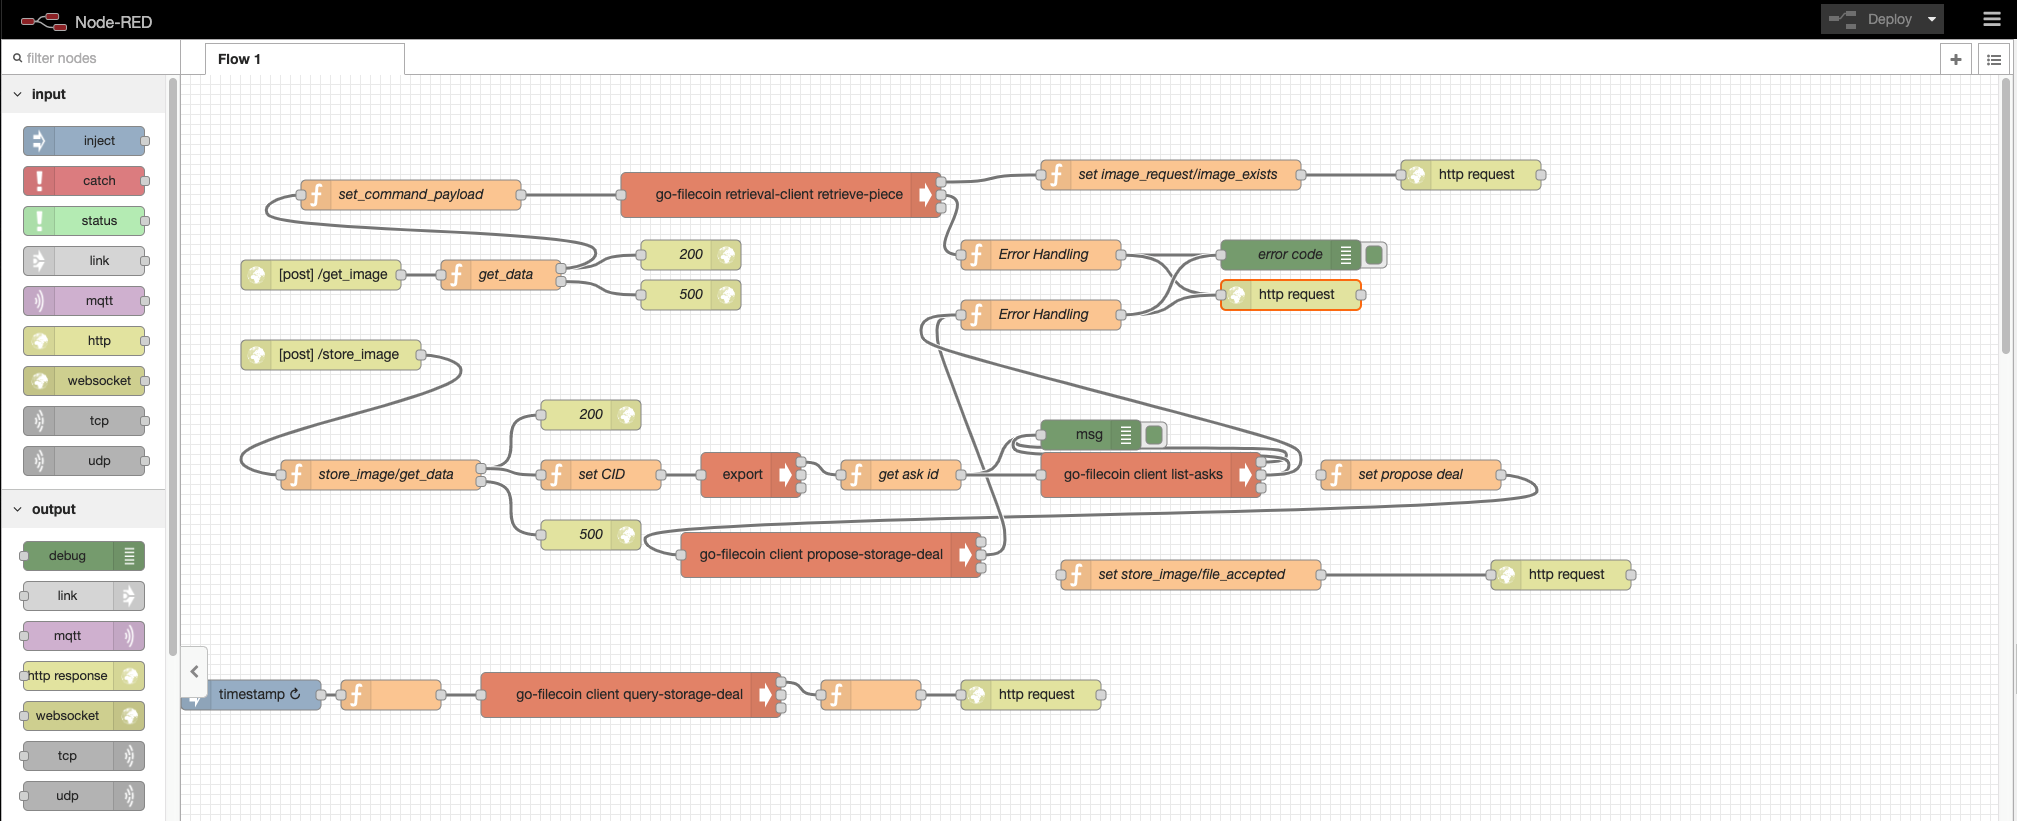
\includegraphics[width=0.9\textwidth]{images/nodered_backend.png}
    \caption{The Filecoin Backend service is a Node-RED instance with a single flow, a RESTful API}
    \label{fig:filecoin_backend}
\end{sidewaysfigure}

Finally we note that we don’t use HTTP to send the images from the edge device to the backend and vice-versa. This is because when uploading using the POST HTTP method (e.g via curl), the whole file is buffered into the memory before being uploaded. This is hugely inefficient, since our Raspberry is extremely memory constrained, taking into consideration the number of services which run concurrently.

Thus, we opted to use \texttt{scp} (secure copy) which can copy files from and to a remote server using the ssh protocol. The file is sent in buffered chunks, thus the memory footprint is kept considerably lower. While this implies trust between the two computers (as we use the same credentials used for ssh), there are methods to make it work (e.g create a user with zero privileges) or we could switch to ftp which is less efficient but still expected to be feasible in our setup.

At a high level, Filecoin Interface sends an image using scp and informs Filecoin backend of the existence of the image. Conversely, when requesting an image, Filecoin interface will request the image from the backend service, the backend service will proceed to download it from the Filecoin DSN and finally it will notify Filecoin Interface so as it uses scp to download it.


